\documentclass[../main.tex]{subfiles}

\graphicspath{../images/}

\begin{document}

\section{Electrostatics}
\barh 

\paragraph{2.1}
(a) Given twelve equal charges, $q$ situated on corners of a regular 12-sided polygon, 
the net force is
\begin{align*}
    \vec{F}_a &= \sum_{i=1}^{12} \frac{1}{4\pi\epsilon_0} 
        \frac{qQ}{\scriptr_{i}^2} \hat \boldscriptr = 0
\end{align*}
since the forces on each pair of charges (e.g., 12 and 6 o' clock) opposite to each other 
cancel out. \\
(b) If one of the charges is removed at 6 o' clock, the net force is strictly due to the the source
charge at 12 o' clock:
\begin{align*}
    \vb{F}_b = \frac{1}{4\pi\epsilon_0} \frac{qQ}{\scriptr_{12}^2} \hat \boldscriptr_{12}
\end{align*}
where $\vb{F}_b$ points from 12 to 6 o' clock. \\
(c) For 13 equal charges, the net force is still $\vb{F}_c = 0$ because the symmetry of the
arrangement is preserved. \\
(d) Removing one of the charges $\vb{r}'_i$ is equivalent to the superposition of a source charge,
$-q$, at $\vb{r}'_i$ and the original configuration. The net force is then
\begin{align*}
    \vb{F}_d = \vb{F}_c - \frac{1}{4\pi\epsilon_0} \frac{qQ}{\scriptr_{i}^2} \hat \boldscriptr_{i}
    = -\frac{1}{4\pi\epsilon_0} \frac{qQ}{\scriptr_{i}^2} \hat \boldscriptr_{i}
\end{align*}

\paragraph{2.2}
\begin{figure}[ht]
    \centering
    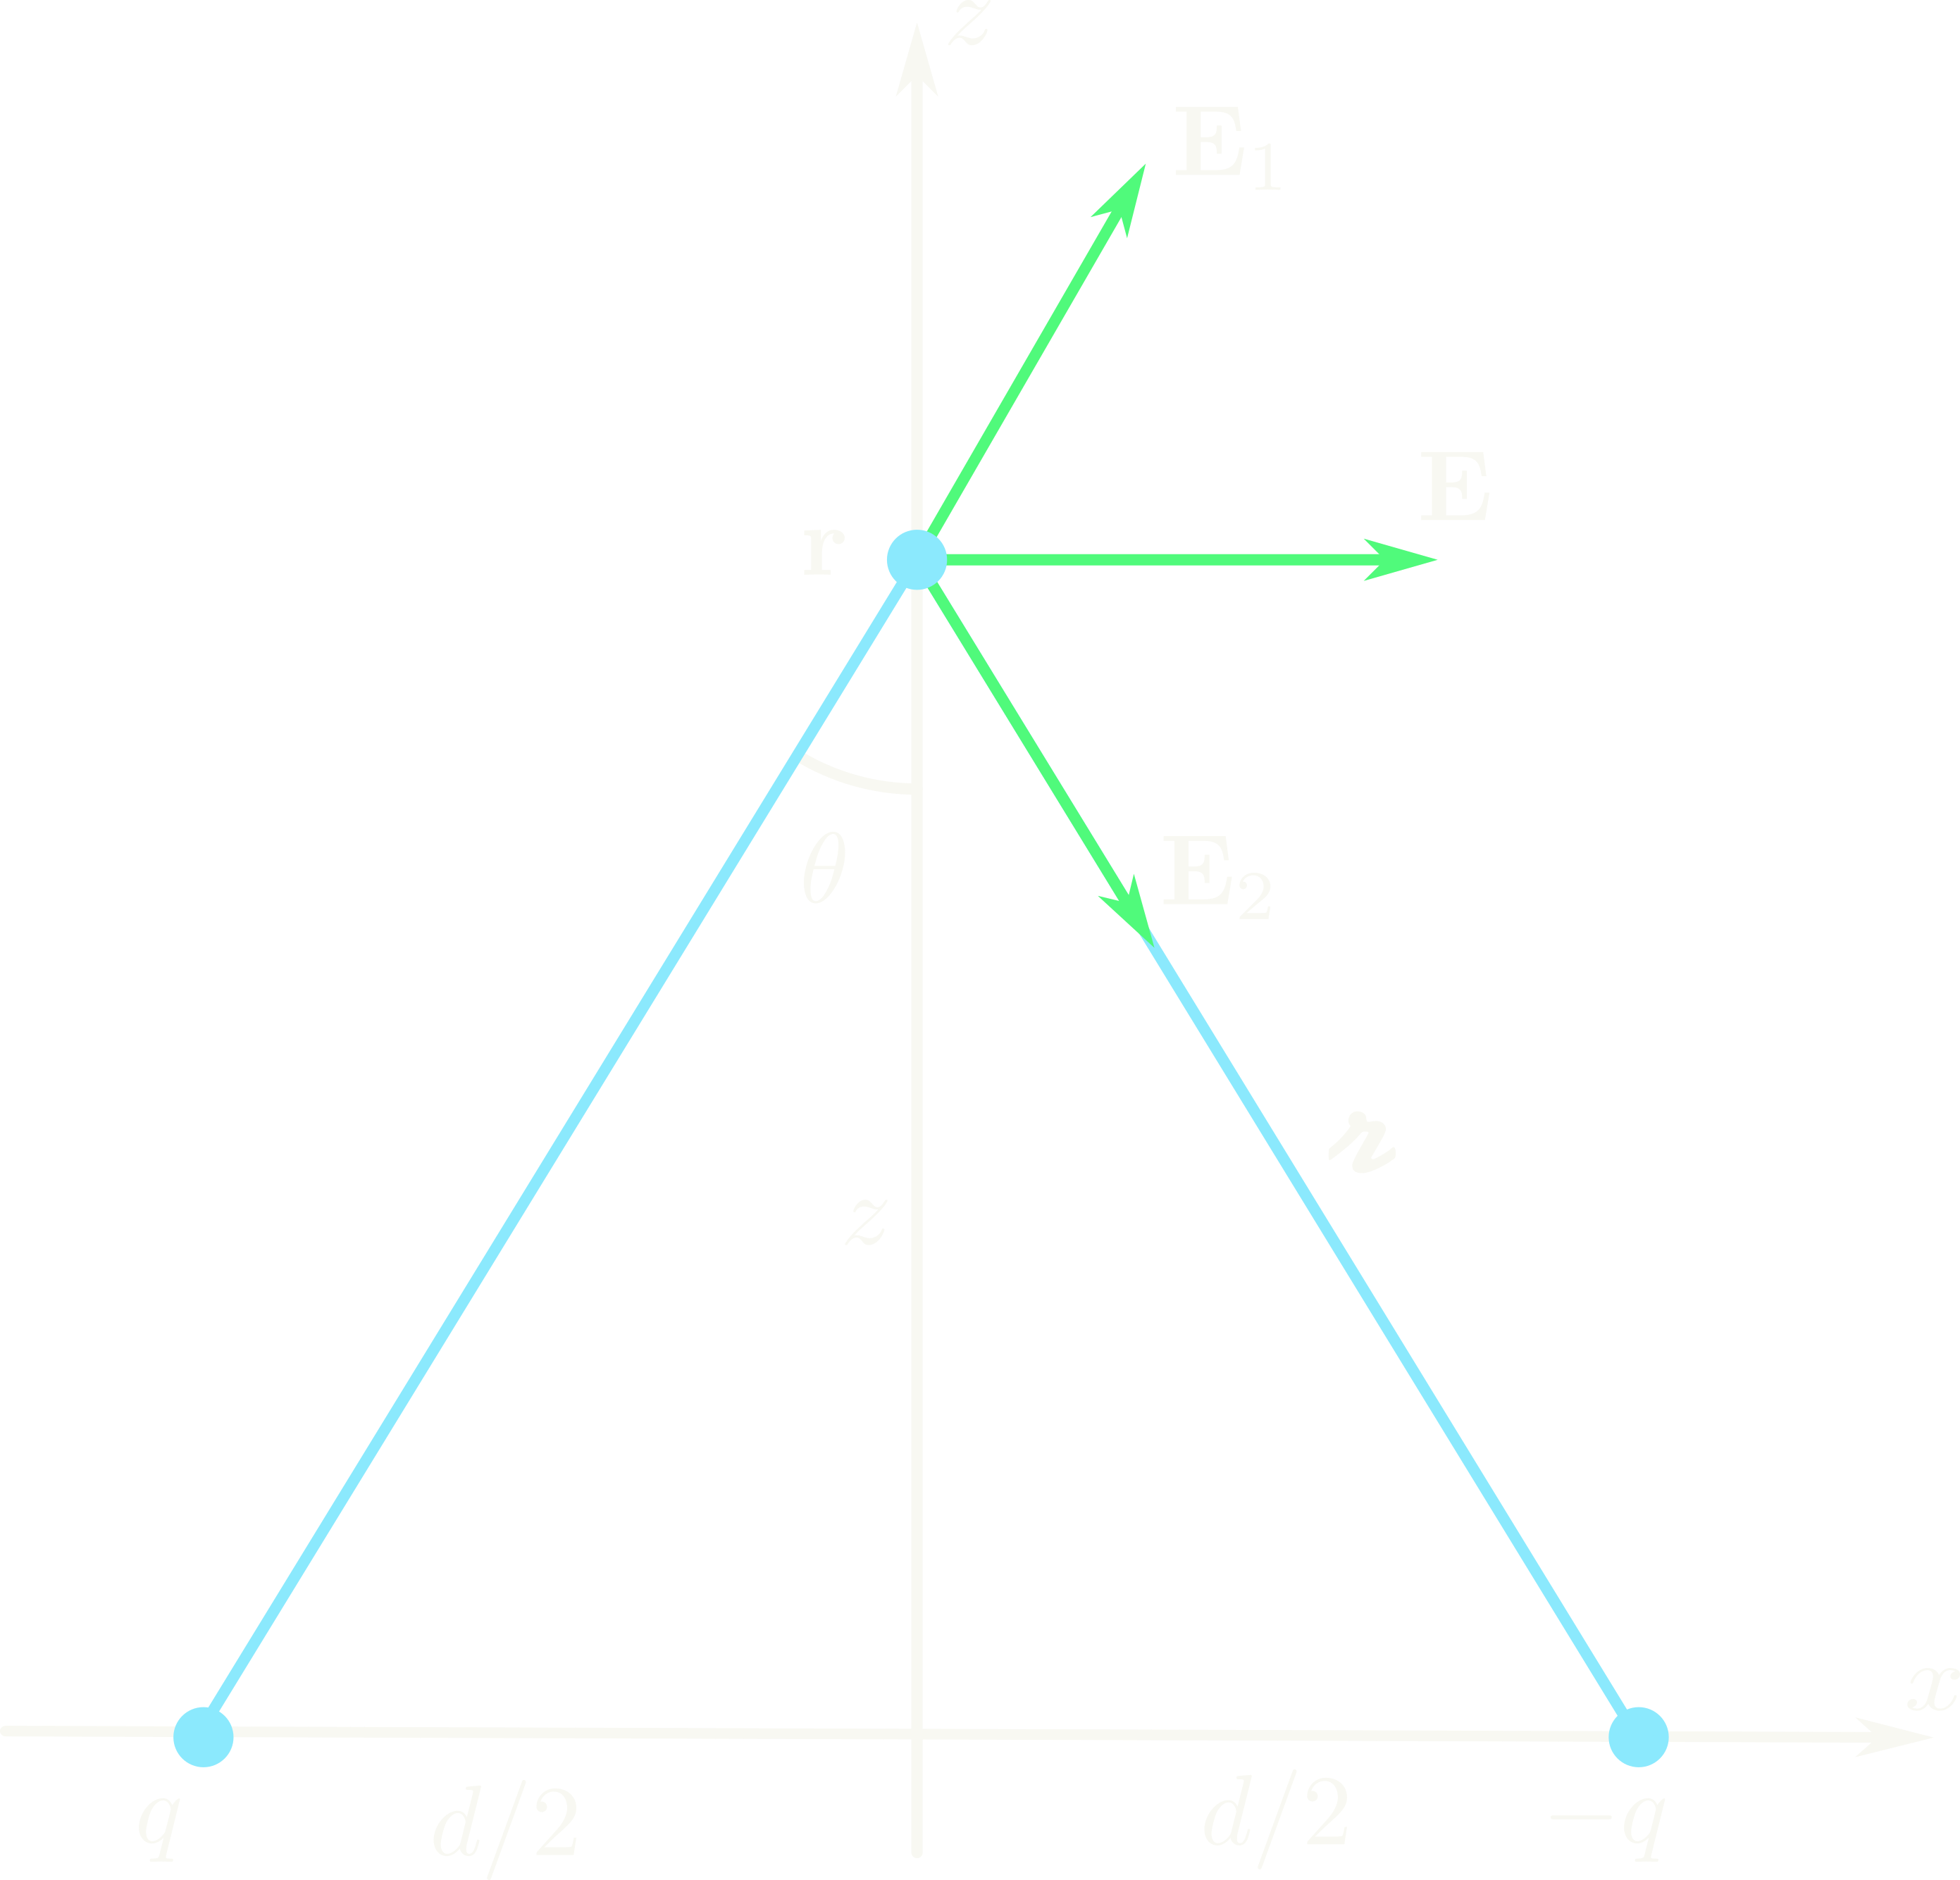
\includegraphics[width=0.5\linewidth]{images/fig2_2.png}
    \captionsetup{width=0.8\linewidth}
    \caption{An electric field at a distance $z$ from the midpoint between equal and opposite
    charges $(\pm q)$ separated by a distance $d$. The charge at $x = d/2$ is $-q$.}
    \label{fig:2_2}
\end{figure}
The vertical componets of the electric field cancel out and the horizontal components add up:
\begin{align*}
    E_x &= 2 \frac{1}{4\pi\epsilon_0} \frac{q}{\scriptr^2} \sin \theta
\end{align*}
where $E_x = E \cos \theta$, $\scriptr = \sqrt{z^2 + (d/2)^2}$, and $\sin \theta = d / (2\scriptr)$,
so 
\begin{align*}
    \vb{E} = \frac{1}{4\pi\epsilon_0} \frac{qd}{[z^2 + (d/2)^2]^{3/2}} \vu{x}
\end{align*}

\paragraph{2.3}
\begin{gather*}
    \vb{r} = z \vu{z} ,\quad \vb{r}' = x \vu{x} ,\quad \dd{l} = \dd{x}; \\
    \boldscriptr = z \vu{z} - x \vu{x} ,\quad \scriptr = \sqrt{z^2 + x^2} ,\quad 
        \hat \boldscriptr = \frac{z \vu{z} - x \vu{x}}{\sqrt{z^2 + x^2}}
\end{gather*}
With uniform line charge $\lambda$ and the limts of integration $[0,L]$,
\begin{align*}
    \vb{E} &= \frac{1}{4\pi\epsilon_0} \int \frac{\lambda \dd{l}}{\scriptr^2} \hat \boldscriptr \\
    &= \frac{\lambda}{4\pi\epsilon_0}
    \int_0^L \frac{z \vu{z} - x \vu{x}}{[z^2 + x^2]^{3/2}} \dd{x} \\
    &= \frac{\lambda}{4\pi\epsilon_0} \qt[
        z \vu{z} \int_0^L \frac{1}{(z^2 + x^2)^{3/2}}
        - \vu{x} \int_0^L \frac{x}{(z^2 + x^2)^{3/2}}
    ] \\
    &= \frac{\lambda}{4\pi\epsilon_0} \qt[
        z \vu{z} \qt(\frac{x}{z^2 \sqrt{z^2 + x^2}}) \eval_0^L
        + \vu{x} \qt(\frac{1}{\sqrt{z^2 + x^2}}) \eval_0^L
    ] \\
    &= \frac{\lambda}{4\pi\epsilon_0} \qt[
        z \vu{z} \qt(\frac{L}{z^2 \sqrt{z^2 + L^2}} - \frac{0}{z^2 \sqrt{z^2 + 0^2}})
        + \vu{x} \qt(\frac{1}{\sqrt{z^2 + L^2}} - \frac{1}{\sqrt{z^2 + 0^2}})
    ] \\
    &= \frac{\lambda}{4\pi\epsilon_0} \qt[
        \vu{z} \qt(\frac{L}{z \sqrt{z^2 + L^2}})
        + \vu{x} \qt(\frac{1}{\sqrt{z^2 + L^2}} - \frac{1}{z})
    ] \\
   \vb{E} &= \frac{1}{4\pi\epsilon_0} \frac{\lambda}{z} \qt[
        \vu{x} \qt(\frac{z}{\sqrt{z^2 + L^2}} - 1) +
        \vu{z} \qt(\frac{L}{\sqrt{z^2 + L^2}})
    ]
\end{align*}
For $z \gg L$,
\begin{align*}
    \vb{E} \approx \frac{1}{4\pi\epsilon_0} \frac{\lambda L}{z^2} \vu{z}
\end{align*}
From far away, the line looks like a point charge $q = \lambda L$.

\paragraph{2.4}
One segment of the square loop is equivalent to Ex. 2.2, but with line segment length $2L \to a$
and electric field distance $z_o \to \sqrt{z_o^2 + a^2/4}$. So, the magnitude of the electric field
from one segment is
\begin{align*}
    E &= \frac{1}{4\pi\epsilon_0} \frac{2\lambda L}{z_o \sqrt{z_o^2 + L^2}} \\
    &= \frac{1}{4\pi\epsilon_0} \frac{\lambda a}{\sqrt{z^2 + a^2/4} \sqrt{z^2 + a^2/2}}  \\
\end{align*}
Due to the symmetry of the loop, the electric field components in the $x$-direction cancel out,
and the electric field components in the $z$-direction add up:
\begin{align*}
    \vb{E} &= 4 E \cos{\theta} \vu{z} \\
    &= \frac{1}{4\pi\epsilon_0} \frac{\lambda a}{\sqrt{z^2 + a^2/4} \sqrt{z^2 + a^2/2}} 
        \frac{z}{\sqrt{z^2 + a^2/4}} \vu{z} \\
    &= \frac{1}{4\pi\epsilon_0} \frac{\lambda a z}{(z^2 + a^2/4) \sqrt{z^2 + a^2/2}} \vu{z}
\end{align*}

\paragraph{2.5}
The horizontal components of the electric field cancel out, and the vertical components conspire:
\begin{align*}
    \vb{E} &= \frac{1}{4\pi\epsilon_0}
        \int \frac{\lambda}{\scriptr^2} \cos\theta \vu{z} \dd{\vb{l}}
\end{align*}
where geometrically $\scriptr = \sqrt{z^2 + r^2}$ and $\cos\theta = z / \scriptr$. So,
\begin{align*}
    \vb{E} &= \frac{1}{4\pi\epsilon_0}
        \int \frac{\lambda z}{(z^2 + r^2)^{3/2}} \vu{z} \dd{\vb{l}}
\end{align*}
and the line integral is over the circumference of the circle, so $\dd{\vb{l}} = r \dd{\theta}$ and
the limits of integration are $[0, 2\pi]$:
\begin{align*}
    \vb{E} &= \frac{1}{4\pi\epsilon_0} \frac{\lambda z}{(z^2 + r^2)^{3/2}} \vu{z}
        \int_0^{2\pi}  r \dd{\theta} \\
    &= \frac{1}{4\pi\epsilon_0}
        \frac{\lambda z (2\pi r)}{(z^2 + r^2)^{3/2}}
\end{align*}

\paragraph{2.6}
The electric field is only in the $z$-direction where $\cos\theta = z/\scriptr$:
\begin{align*}
    \vb{E} &= \frac{1}{4\pi\epsilon_0}
        \int \frac{\sigma}{\scriptr^2} \cos\theta \vu{z} \dd{\vb{a}} \\
    &= \frac{1}{4\pi\epsilon_0}
        \int \frac{\sigma z}{(z^2 + r^2)^{3/2}} \vu{z} \dd{\vb{a}}
\end{align*}
Using polar coordinates: since $\dd{\vb{a}} = r \dd{r} \dd{\theta} $
\begin{align*}
    \vb{E} &= \frac{1}{4\pi\epsilon_0}
        \int_0^{2\pi} \int_0^R \frac{\sigma z}{(z^2 + r^2)^{3/2}} \vu{z} r \dd{r} \dd{\theta} \\
    &= \frac{1}{4\pi\epsilon_0}
        \sigma z (2\pi) \vu{z} \int_0^R \frac{r}{(z^2 + r^2)^{3/2}} \dd{r} \\
    &= \frac{\sigma}{2\epsilon_0} z \vu{z} \qt[
            -\frac{1}{\sqrt{z^2 + r^2}}
        ]_0^R \\
    &= \frac{\sigma}{2\epsilon_0} z  \qt[
            \frac{1}{z} -\frac{1}{\sqrt{z^2 + R^2}}
        ] \vu{z} \\
    \vb E &= \frac{\sigma}{2\epsilon_0} \qt[1 - \frac{1}{\sqrt{z^2 + R^2}}] \vu{z}
\end{align*}
when $R \to \infty$,
\begin{align*}
    \vb{E} &= \frac{1}{4\pi\epsilon_0} 2\pi \sigma \vu{z} = \frac{\sigma}{2\epsilon_0} \vu{z}
\end{align*}
for $z \gg R$,
\begin{align*}
    -\frac{1}{\sqrt{z^2 + R^2}} = -\frac{1}{z} \qt(1 + \frac{R^2}{z^2})^{-1/2} \approx -\frac{1}{z}
    \qt(1 - \frac{1}{2} \frac{R^2}{z^2}) = -\frac{1}{z} + \frac{1}{2} \frac{R^2}{z^3}
\end{align*}
where the binomial theorem approximation $(1 + x)^n \approx 1 + nx$ is used. So,
\begin{align*}
    \vb{E} = \frac{1}{4\pi\epsilon_0} 2\pi \sigma z \qt[
        \frac{1}{z} - \frac{1}{z} + \frac{1}{2} \frac{R^2}{z^3}
    ] \vu{z} 
    = \frac{1}{4\pi\epsilon_0} \frac{\pi R^2 \sigma }{z^2} \vu{z}
\end{align*}
or a point charge $q = \pi R^2 \sigma$ from far away.
\newpage
\paragraph{2.7}
\begin{figure}[ht]
    \centering
    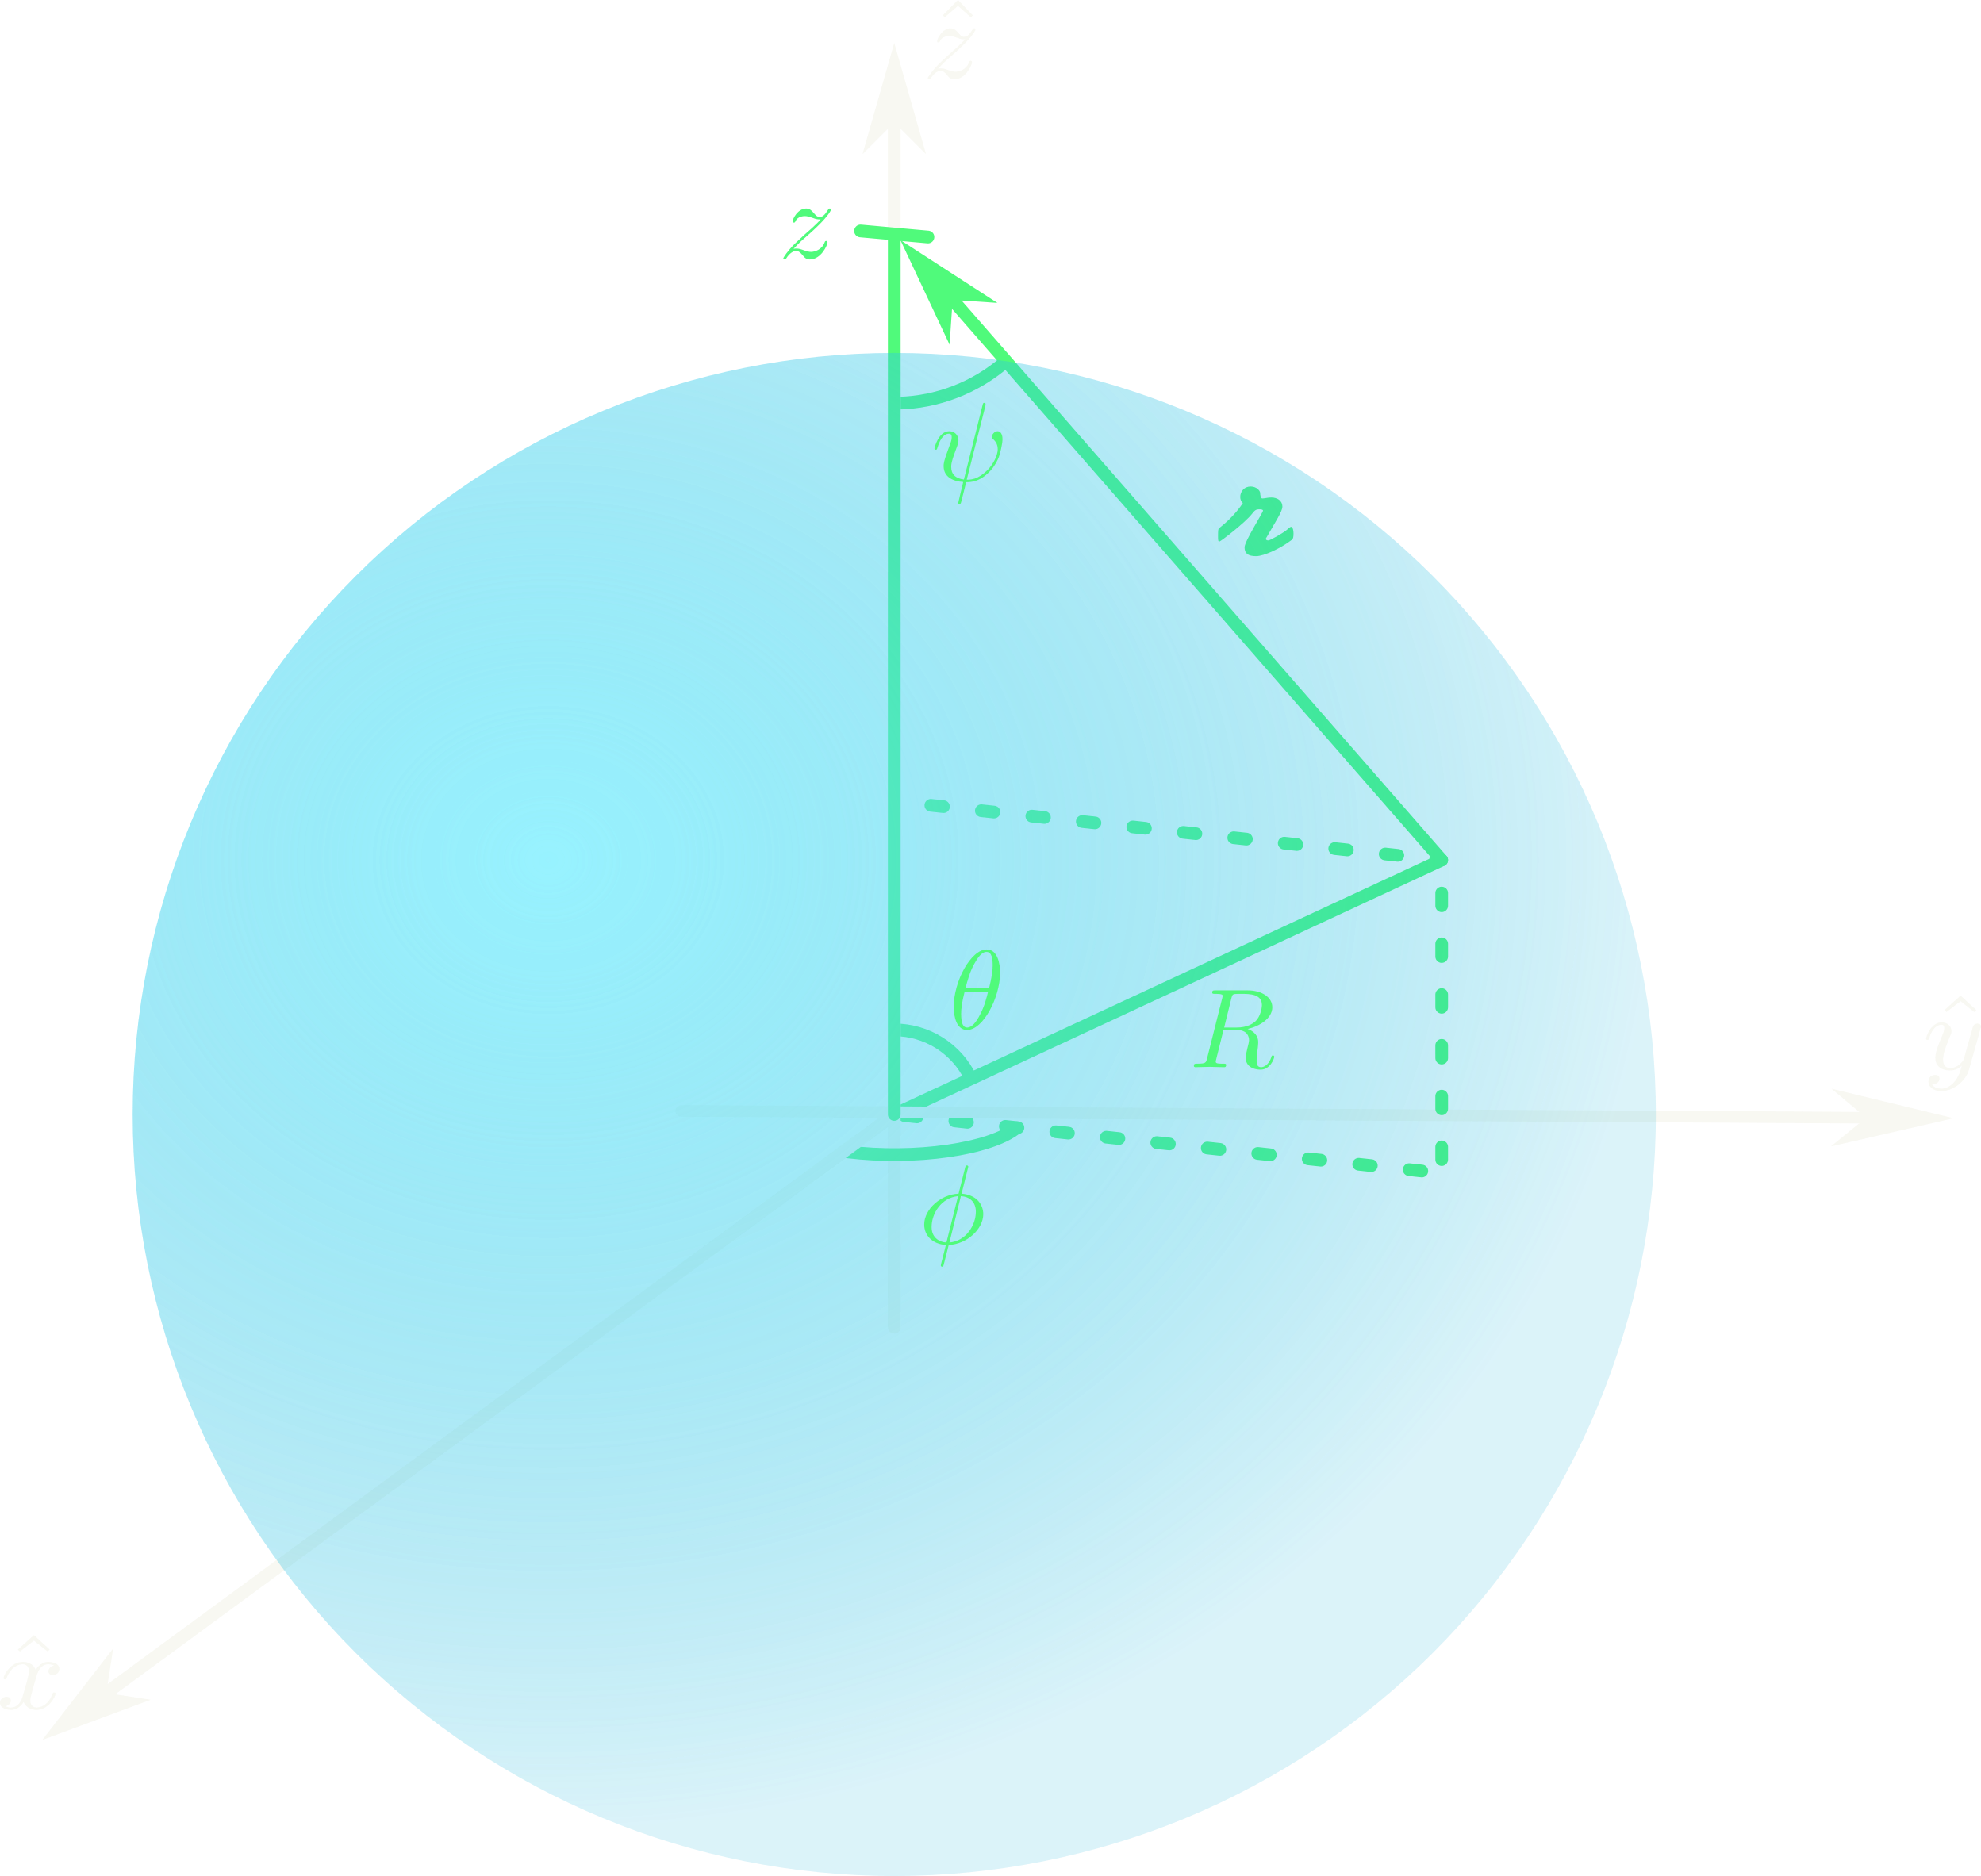
\includegraphics[width=0.5\linewidth]{images/fig2_7.png}
    \captionsetup{width=0.8\linewidth}
    \caption{An electric field a distance $z$ from the center of a spherical surface of radius $R$
    that carries a charge density $\sigma$.}
    \label{fig:2_7}
\end{figure}
Once again, the electric field is in the $z$-direction:
\begin{equation}
    \vb{E} = \frac{1}{4\pi\epsilon_0}   
    \int \frac{\sigma}{\scriptr^2} \cos\psi \vu{z} \dd{\vb{a}}
\end{equation}
From the law of cosines, $\scriptr^2 = z^2 + R^2 - 2zR\cos\theta$; Geometrically,
$\cos\psi = \dfrac{z - R \cos\theta}{\scriptr}$; the surface area element is
$\dd{\vb{a}} = R^2 \sin\theta \dd{\theta} \dd{\theta}$:
\begin{align*}
    \vb{E} &=  \ke\int_0^{2\pi} \int_0^{\pi}
        \frac{\sigma R^2(z - R \cos\theta)}{(z^2 + R^2 - 2zR\cos\theta)^{3/2}}
        \sin\theta \dd{\theta} \dd{\phi} \vu{z} \\
        &= \ke (2\pi\sigma R^2) \int_0^{\pi}
        \frac{z - R \cos\theta}{(z^2 + R^2 - 2zR\cos\theta)^{3/2}}
        \sin\theta \dd{\theta} \vu{z} \\
        &= \ke (2\pi\sigma R^2) f(\theta) \vu{z}
\end{align*}
using the substitution $u = \cos\theta$: $\dd{u} = -\sin\theta \dd{\theta}$, and the limits of
integration are $[\cos{0}, \cos{\pi}]$. So,
\begin{align*}
    f(\theta) =
    \int_{-1}^{1} \frac{z - Ru}{(z^2 + R^2 - 2zRu)^{3/2}} \dd{u} = f(u)
\end{align*}
substituting again with $v = \sqrt{z^2 + R^2 - 2zRu}$; $\dd{v} = -\dfrac{zR}{v} \dd{u}$; and $
u = \dfrac{1}{2zR}(z^2 + R^2 - v^2)$:
\begin{align*}
    f(v) &= -\frac{1}{zR} \int \frac{z - \frac{1}{2z}(z^2 + R^2 - v^2)}{v^3} v \dd{v} \\
    &= -\frac{1}{2z^2R} \int \frac{2z^2 - (z^2 + R^2 - v^2)}{v^2} \dd{v} \\
    &= -\frac{1}{2z^2R} \int \frac{v^2 + z^2 - R^2}{v^2} \dd{v} \\
    &= -\frac{1}{2z^2R} \int \qt(1 + \frac{z^2 - R^2}{v^2}) \dd{v} \\
    &= -\frac{1}{2z^2R} \qt(v - \frac{z^2 - R^2}{v})
\end{align*}
back substituting $v = \sqrt{z^2 + R^2 - 2zRu}$,
\begin{align*}
    f(u) &= -\frac{1}{2z^2R} \qt(\frac{z^2 + R^2 - 2zRu}{\sqrt{z^2+R^2-2zRu}} 
        - \frac{z^2 - R^2}{\sqrt{z^2 + R^2 - 2zRu}}) \eval_{-1}^1 \\
    &= -\frac{1}{2z^2R} \qt(\frac{2R^2 - 2zRu}{\sqrt{z^2+R^2-2zRu}}) \eval_{-1}^1 \\
    &= \frac{1}{z^2} \qt(\frac{zu - R}{\sqrt{z^2+R^2-2zRu}}) \eval_{-1}^1 \\
    &= \frac{1}{z^2} \qt(
        \frac{z - R}{\sqrt{z^2 + R^2 - 2zR}} - \frac{-z - R}{\sqrt{z^2 + R^2 + 2zR}}
    )
\end{align*}
Taking the positive square root: $\sqrt{z^2 + R^2 - 2zR} = (R - z)$ if $R > z$, but $(z - R)$ if
$R < z$. So, for the case $z < R$ (inside the sphere) the electric field is
\begin{align*}
    \vb{E} &= \frac{1}{4\pi\epsilon_0} \frac{2\pi\sigma R^2}{z^2} \qt(
        \frac{z - R}{R - z} - \frac{-z - R}{R + z}
    ) \vu{z} \\
    &= \frac{1}{4\pi\epsilon_0} \frac{2\pi\sigma R^2}{z^2} \qt(
        \frac{z - R}{R - z} + \frac{z + R}{R + z}
    ) \vu{z} \\
    &= \frac{1}{4\pi\epsilon_0} \frac{2\pi\sigma R^2}{z^2} \qt(
        \frac{z - R}{R - z} + 1
    ) \vu{z} \\
    &= \frac{1}{4\pi\epsilon_0} \frac{2\pi\sigma R^2}{z^2} \qt(
        \frac{z - R}{R - z} + \frac{R - z}{R - z}
    ) \vu{z} \\
    &= 0
\end{align*}
For the case $z > R$ (outside the sphere) the electric field is
\begin{align*}
    \vb{E} &= \ke \frac{2\pi\sigma R^2}{z^2} \qt(
        \frac{z - R}{z - R} + \frac{z + R}{z + R}
    ) \vu{z} \\
    &= \ke \frac{4\pi\sigma R^2}{z^2} \vu{z} \\
    &= \ke \frac{q}{z^2} \vu{z}
\end{align*}
This makes sense: From outside the sphere, the point charge $q$ is the
charge-per-area $\sigma$ times the surface area of the sphere $4\pi R^2$, or simply
$q = 4\pi R^2 \sigma$.

\paragraph{2.8}\label{prob:2_8}
Finding the field inside and outside a solid sphere of radius $R$ with a uniform volume charge
density $\rho$ is similar to Prob. 2.7. Outside the solid sphere the total charge $q$ contributes
to the electric field as if it were a point charge:
\begin{align*}
    \vb{E}_{out} &= \ke \frac{q}{r^2} \vu{r}
\end{align*}
Inside the solid sphere, only the volume of the solid sphere less than $r$ contributes to the
electric field. The volume of the total sphere is $V = \frac{4}{3}\pi R^3$, and the volume of the
sphere less than $r$ is $V' = \frac{4}{3}\pi r^3$. So, electric field inside the solid sphere is
\begin{align*} 
    \vb{E}_{in} &= \frac{V'}{V} \vb{E}_{out} \\
    &= \frac{r^3}{R^3} \ke \frac{q}{r^2} \vu{r} \\
    &= \ke \frac{q}{R^3} r \vu{r} 
\end{align*}
or
\begin{align*}
    \vb{E}_{in} = \ke \frac{q}{R^3} \vb{r}
\end{align*}

\paragraph{2.9}
(a) The electric field in some region is $\vb{E} = kr^3 \vu{r}$ in spherical coordinates, where
$k$ is a constant. The differential form of Gauss's law is
\begin{align*}
    \div{\vb{E}} &= \frac{\rho}{\epsilon_0}
\end{align*}
and the radial component of divergence in spherical coordinates is
\begin{align*}
    [\div{\vb{E}}]_r &= \frac{1}{r^2} \pdv{r} (r^2 E_r) \\
    &= \frac{1}{r^2} \pdv{r} (r^2 kr^3) \\
    &= 5kr^2
\end{align*}
So, the charge density is
\begin{align*}
    \rho &= 5\epsilon_0 kr^2
\end{align*}
(b) The total charge inside a sphere of radius $R$ is found using Gauss's law:
\begin{align*}
\oint \vb{E} \vdot \dd{\vb{a}} &= \frac{Q}{\epsilon_o} \\
Q &= \epsilon_o \oint \vb{E} \vdot \dd{\vb{a}} \\
&= \epsilon_o \int (kR^3 \vu{r}) \vdot (R^2 \sin\theta \dd{\theta} \dd{\phi} \vu{r}) \\
&= \epsilon_o \int_0^{2\pi} \int_0^\pi (kR^5 \sin\theta) \dd{\theta} \dd{\phi} \\
&= 4\pi \epsilon_o k R^5
\end{align*}
or using Gauss's theorem:
\begin{align*}
    \oint \vb{E} \vdot \dd{\vb{a}} &= \int (\div \vb{E}) \dd{\tau} \\
    Q &= \epsilon_o \int_0^{2\pi} \int_0^\pi \int_0^R
        5kr^2 (r^2 \sin\theta) \dd{r} \dd{\theta} \dd{\phi} \\
    &= 4\pi \epsilon_o k R^5
\end{align*}

\paragraph{2.10}
For simplicity, using a cube of length 1:
\begin{align*}
    y = 1 ,\quad \vb{E} = \ke \frac{q(x\vu{x} + y\vu{y} + z\vu{z})}{r^3}
    ,\quad \dd{a} = \dd{x} \dd{z} \vu{y} ;\quad \vb{E} \vdot \dd{a} = \ke \frac{q}{r^3}
\end{align*}
the limits of integration are $x = [0,1]$ and $z = [0,1]$:
\begin{align*}
    \oint \vb{E} \vdot \dd{a} &=\ke q \int \frac{1}{r^3} \dd{x} \dd{z} \\
    &= \ke q \int_0^1 \int_0^1 \frac{1}{(x^2 + 1 + z^2)^{3/2}} \dd{x} \dd{z} \\
    &= \ke q \int_0^1 \qt[
        \frac{x}{(1+z^2) \sqrt{x^2 + 1 + z^2}} \eval_0^1 
    ] \dd{z} \\
    &= \ke q \int_0^1 \frac{1}{(1 + z^2) \sqrt{2 + z^2}} \dd{z} \\
    &= \ke q \arctan(\frac{z}{\sqrt{z^2 + 2}}) \eval_0^1 \\
    &= \ke q \qt(\frac{\pi}{6}) = \frac{q}{24\epsilon_o}
\end{align*}
Where the first integral is solved using the trig identity $x = \tan(u) \sqrt{z^2 + 1}$, and 
similarly, the second integral uses $z = \tan(u) \sqrt{2}$.

\begin{figure}[ht]
    \centering
    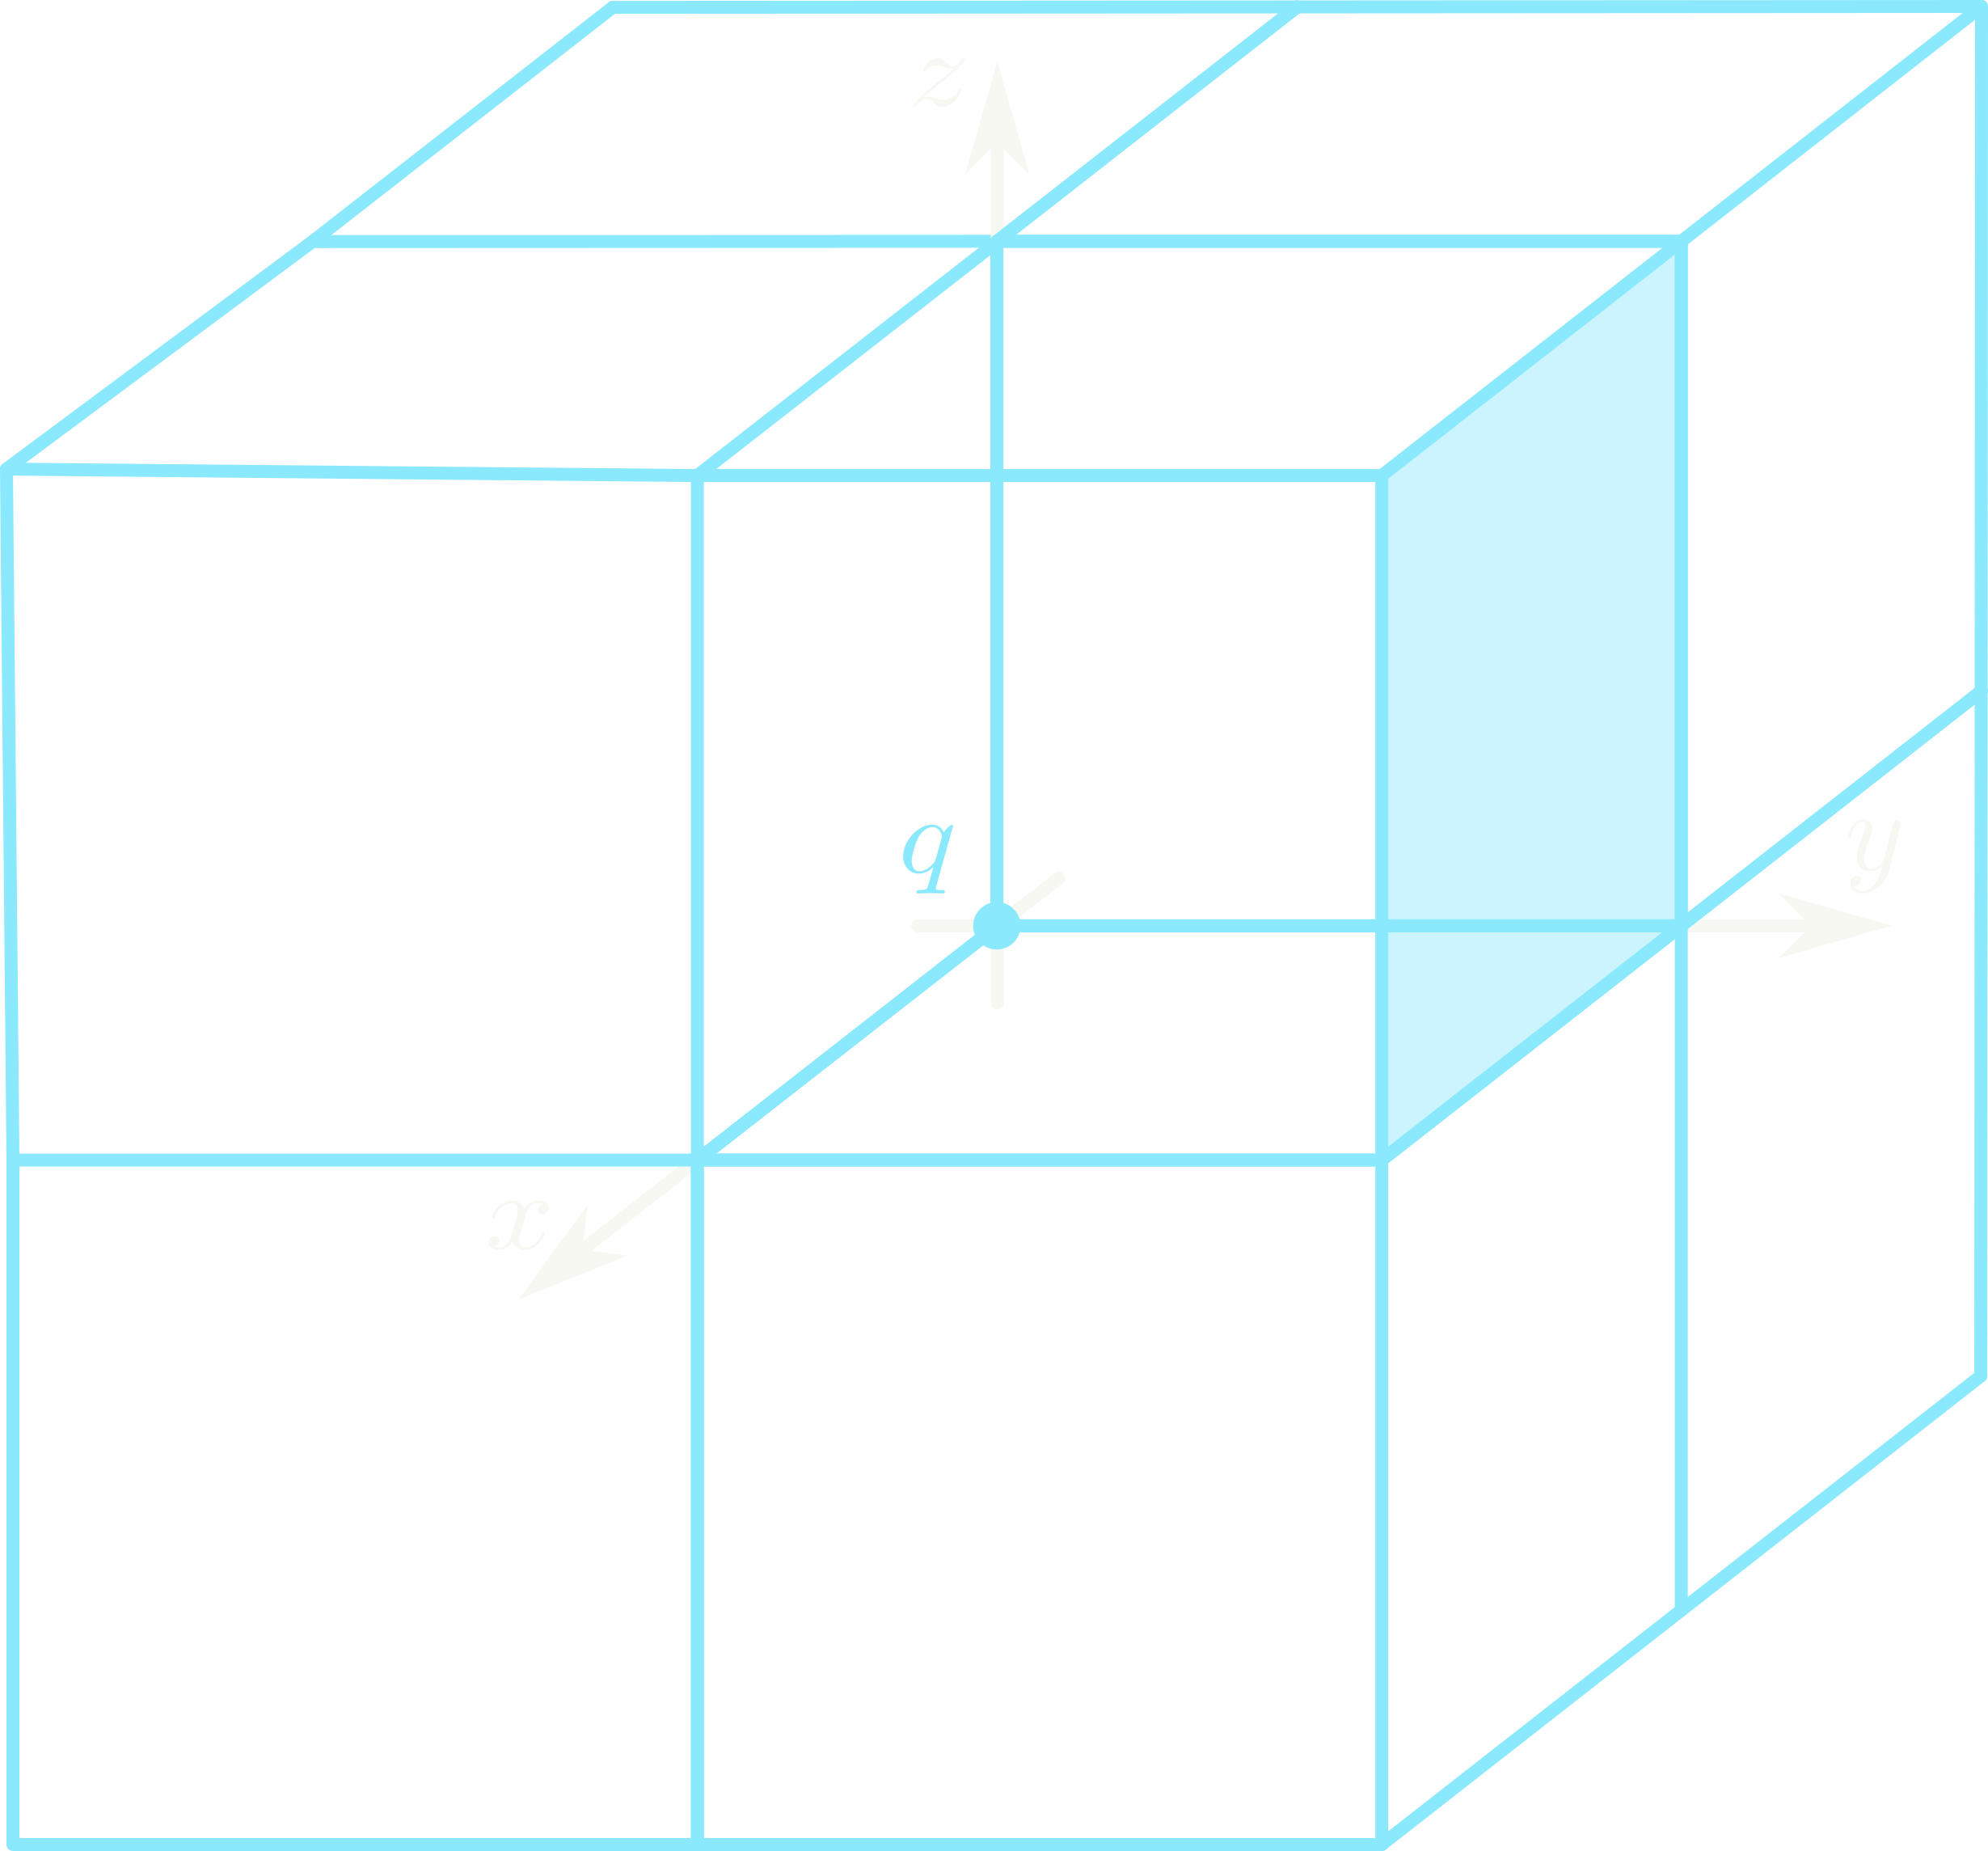
\includegraphics[width=0.5\linewidth]{images/fig2_10.png}
    \captionsetup{width=0.8\linewidth}
    \caption{8 cubes with a charge $q$ at the center.}
    \label{fig:2_10}
\end{figure}
The simpler solution is though the superposition of 8 cubes with the charge in the center of the
larger cube, and the surface that encloses the larger cube is made of 24 squares equivalent to the
shaded region as shown in Figure \ref{fig:2_10}. Therefore, the flux through the shaded region is
$\frac{1}{24}$ of the total flux $\frac{q}{\epsilon_o}$.

\paragraph{2.11}
For a spherical shell of radius $R$ with a uniform surface charge density $\sigma$, the enclosed
charge in side the sphere is $Q_{enc} = 0$, thus the electric field inside the sphere is 
\begin{align*}
    \vb{E}_i = 0
\end{align*}
and using the sphericla symmetry of a Gaussian surface, the electric field outside the sphere is
\begin{align*}
    \oint \vb{E}_o \vdot \dd{\vb{a}} &= \frac{1}{\epsilon_o} Q_{enc} \\
    \abs{\vb{E}_0} \int \dd{\vb{a}} &= \frac{1}{\epsilon_o} (4\pi\sigma R^2) \\
    \vb{E}_o (4\pi r^2) &= \frac{1}{\epsilon_o} (4\pi\sigma R^2) \vu{r} \\
    \vb{E}_o &= \frac{\sigma R^2}{\epsilon_o r^2} \vu{r}
\end{align*}

\paragraph{2.12}
Inside a solid sphere, the total charge enclosed in the Gaussian surface is
\begin{align*}
    Q_{enc} &=  V'\rho = \frac{4}{3} \pi r^3 \rho
\end{align*}
where $V'$ is the volume of the sphere enclosed by the Gaussian surface. Using Gauss's law,
\begin{align*}
    \oint \vb{E} \vdot \dd{\vb{a}} = \frac{1}{\epsilon_o} Q_{enc}
    = \frac{1}{\epsilon_o} \frac{4}{3} \pi r^3 \rho
\end{align*}
using the spherical symmetry of the Gaussian surface, the electric field is
\begin{align*}
    \oint \vb{E} \vdot \dd{\vb{a}} = \abs{\vb{E}} \int \dd{a} 
    = \abs{\vb{E}} (4\pi r^2)
\end{align*}
Thus
\begin{align*}
    \abs{\vb{E}} (4\pi r^2) = \frac{1}{\epsilon_o} \frac{4}{3} \pi r^3 \rho
\end{align*}
or
\begin{align*}
    \vb{E} = \frac{1}{3\epsilon_o} r \rho \vu{r} = \frac{1}{3\epsilon_o} \rho \vb{r}
\end{align*}
Since the total charge of the solid sphere is $q = \frac{4}{3} \pi R^3 \rho$, the electric field
can be rewritten as
\begin{align*}
    \vb{E} = \ke \frac{q}{R^3} \vb{r}
\end{align*}
which is the same as Prob. 2.8.

\paragraph{2.13} \label{prob:2_13}
Finding the electric field a distance $s$ from an infinitely long straight wire that carries a
uniform line charge $\lambda$. Using a Gaussian cylinder of radius $s$ and length $L$, 
enclosed charge is $Q_{enc} = \lambda L$. Using Gauss's law and the symmetry of the cylinder,
\begin{align*}
    \oint \vb{E} \vdot \dd{\vb{a}} &= \frac{1}{\epsilon_o} Q_{enc} \\
    \abs{\vb{E}} \int \dd{s'}\dd{\phi'}\dd{z'} &= \frac{1}{\epsilon_o} \lambda L \\
    E (2\pi s L) &= \frac{1}{\epsilon_o} \lambda L
\end{align*}
or
\begin{align*}
    \vb{E} = \frac{\lambda}{2\pi\epsilon_o s} \vu{s} = \ke \frac{2\lambda}{s} \vu{s}
\end{align*}
which is similar to Eq. 2.9.

\paragraph{2.14}
Find the electric field inside a sphere that carries a charge density proportional to the distance
from the origin, $\rho = kr$, where $k$ is a constant: The enclosed charge is
\begin{align*}
    Q_{enc} = \int \rho \dd{\tau} = \int_0^{2\pi} \int_0^\pi \int_0^r kr (r^2 \sin\theta) \dd{r}
        \dd{\theta} \dd{\phi} = \pi k r^4
\end{align*}
Using Gauss's law and the spherical symmetry of the Gaussian surface,
\begin{align*}
    \oint \vb{E} \vdot \dd{\vb{a}} &= \frac{1}{\epsilon_o} Q_{enc} \\
    \abs{\vb{E}} \int \dd{a} &= \frac{1}{\epsilon_o} \pi k r^4 \\
    E (4\pi r^2) &= \frac{1}{\epsilon_o} \pi k r^4
\end{align*}
or 
\begin{align*}
    \vb{E} = \frac{1}{4\pi\epsilon_o} \pi k r^2 \vu{r} = \ke kr\vb{r}
\end{align*}

\paragraph{2.15} \label{prob:2_15}
A thick spherical shell with charge density
\begin{align*}
    \rho = \frac{k}{r^2} \quad (a\leq r \leq b)
\end{align*}
The electric field in the three regions: \\
(i) \(r<a\)
\[ Q_{enc} = 0; \vb{E} = 0 \]

(ii) \(a\leq r \leq b\)
\[ Q_{enc} = \int_0^{2\pi} \int_0^\pi \int_a^r \rho (r^2 \sin\theta) \dd{r} \dd{\theta} \dd{\phi}
= 4\pi \int_a^r \frac{k}{r^2} (r^2) \dd{r} = 4\pi k (r - a) \]
And from Gauss's law,
\begin{align*}
    \oint \vb{E} \vdot \dd{\vb{a}} &= \frac{1}{\epsilon_o} Q_{enc} \\
    \abs{\vb{E}} \int \dd{a} &= \frac{1}{\epsilon_o} 4\pi k (r - a) \\
    E (4\pi r^2) &= \frac{1}{\epsilon_o} 4\pi k (r - a)
\end{align*}
or 
\begin{align*}
    \vb{E} &= \frac{k (r - a)}{\epsilon_o r^2} \vu{r} = \ke \frac{4\pi k(r - a)}{r^3} \vb{r}
\end{align*}

(iii) \(r>b\)
\[ Q_{enc} = \int_0^{2\pi} \int_0^\pi \int_a^b \rho (r^2 \sin\theta) \dd{r} \dd{\theta} \dd{\phi}
= 4\pi k (b - a) \]
And from Gauss's law,
\begin{align*}
    \oint \vb{E} \vdot \dd{\vb{a}} &= \frac{1}{\epsilon_o} Q_{enc} \\
    \abs{\vb{E}} \int \dd{a} &= \frac{1}{\epsilon_o} 4\pi k (b - a) \\
    E (4\pi r^2) &= \frac{1}{\epsilon_o} 4\pi k (b - a)
\end{align*}
or
\begin{align*}
    \vb{E} &= \frac{k (b - a)}{\epsilon_o r^2} \vu{r} = \ke \frac{4\pi k(b - a)}{r^3} \vb{r}
\end{align*}
\begin{figure}[ht]
    \centering
    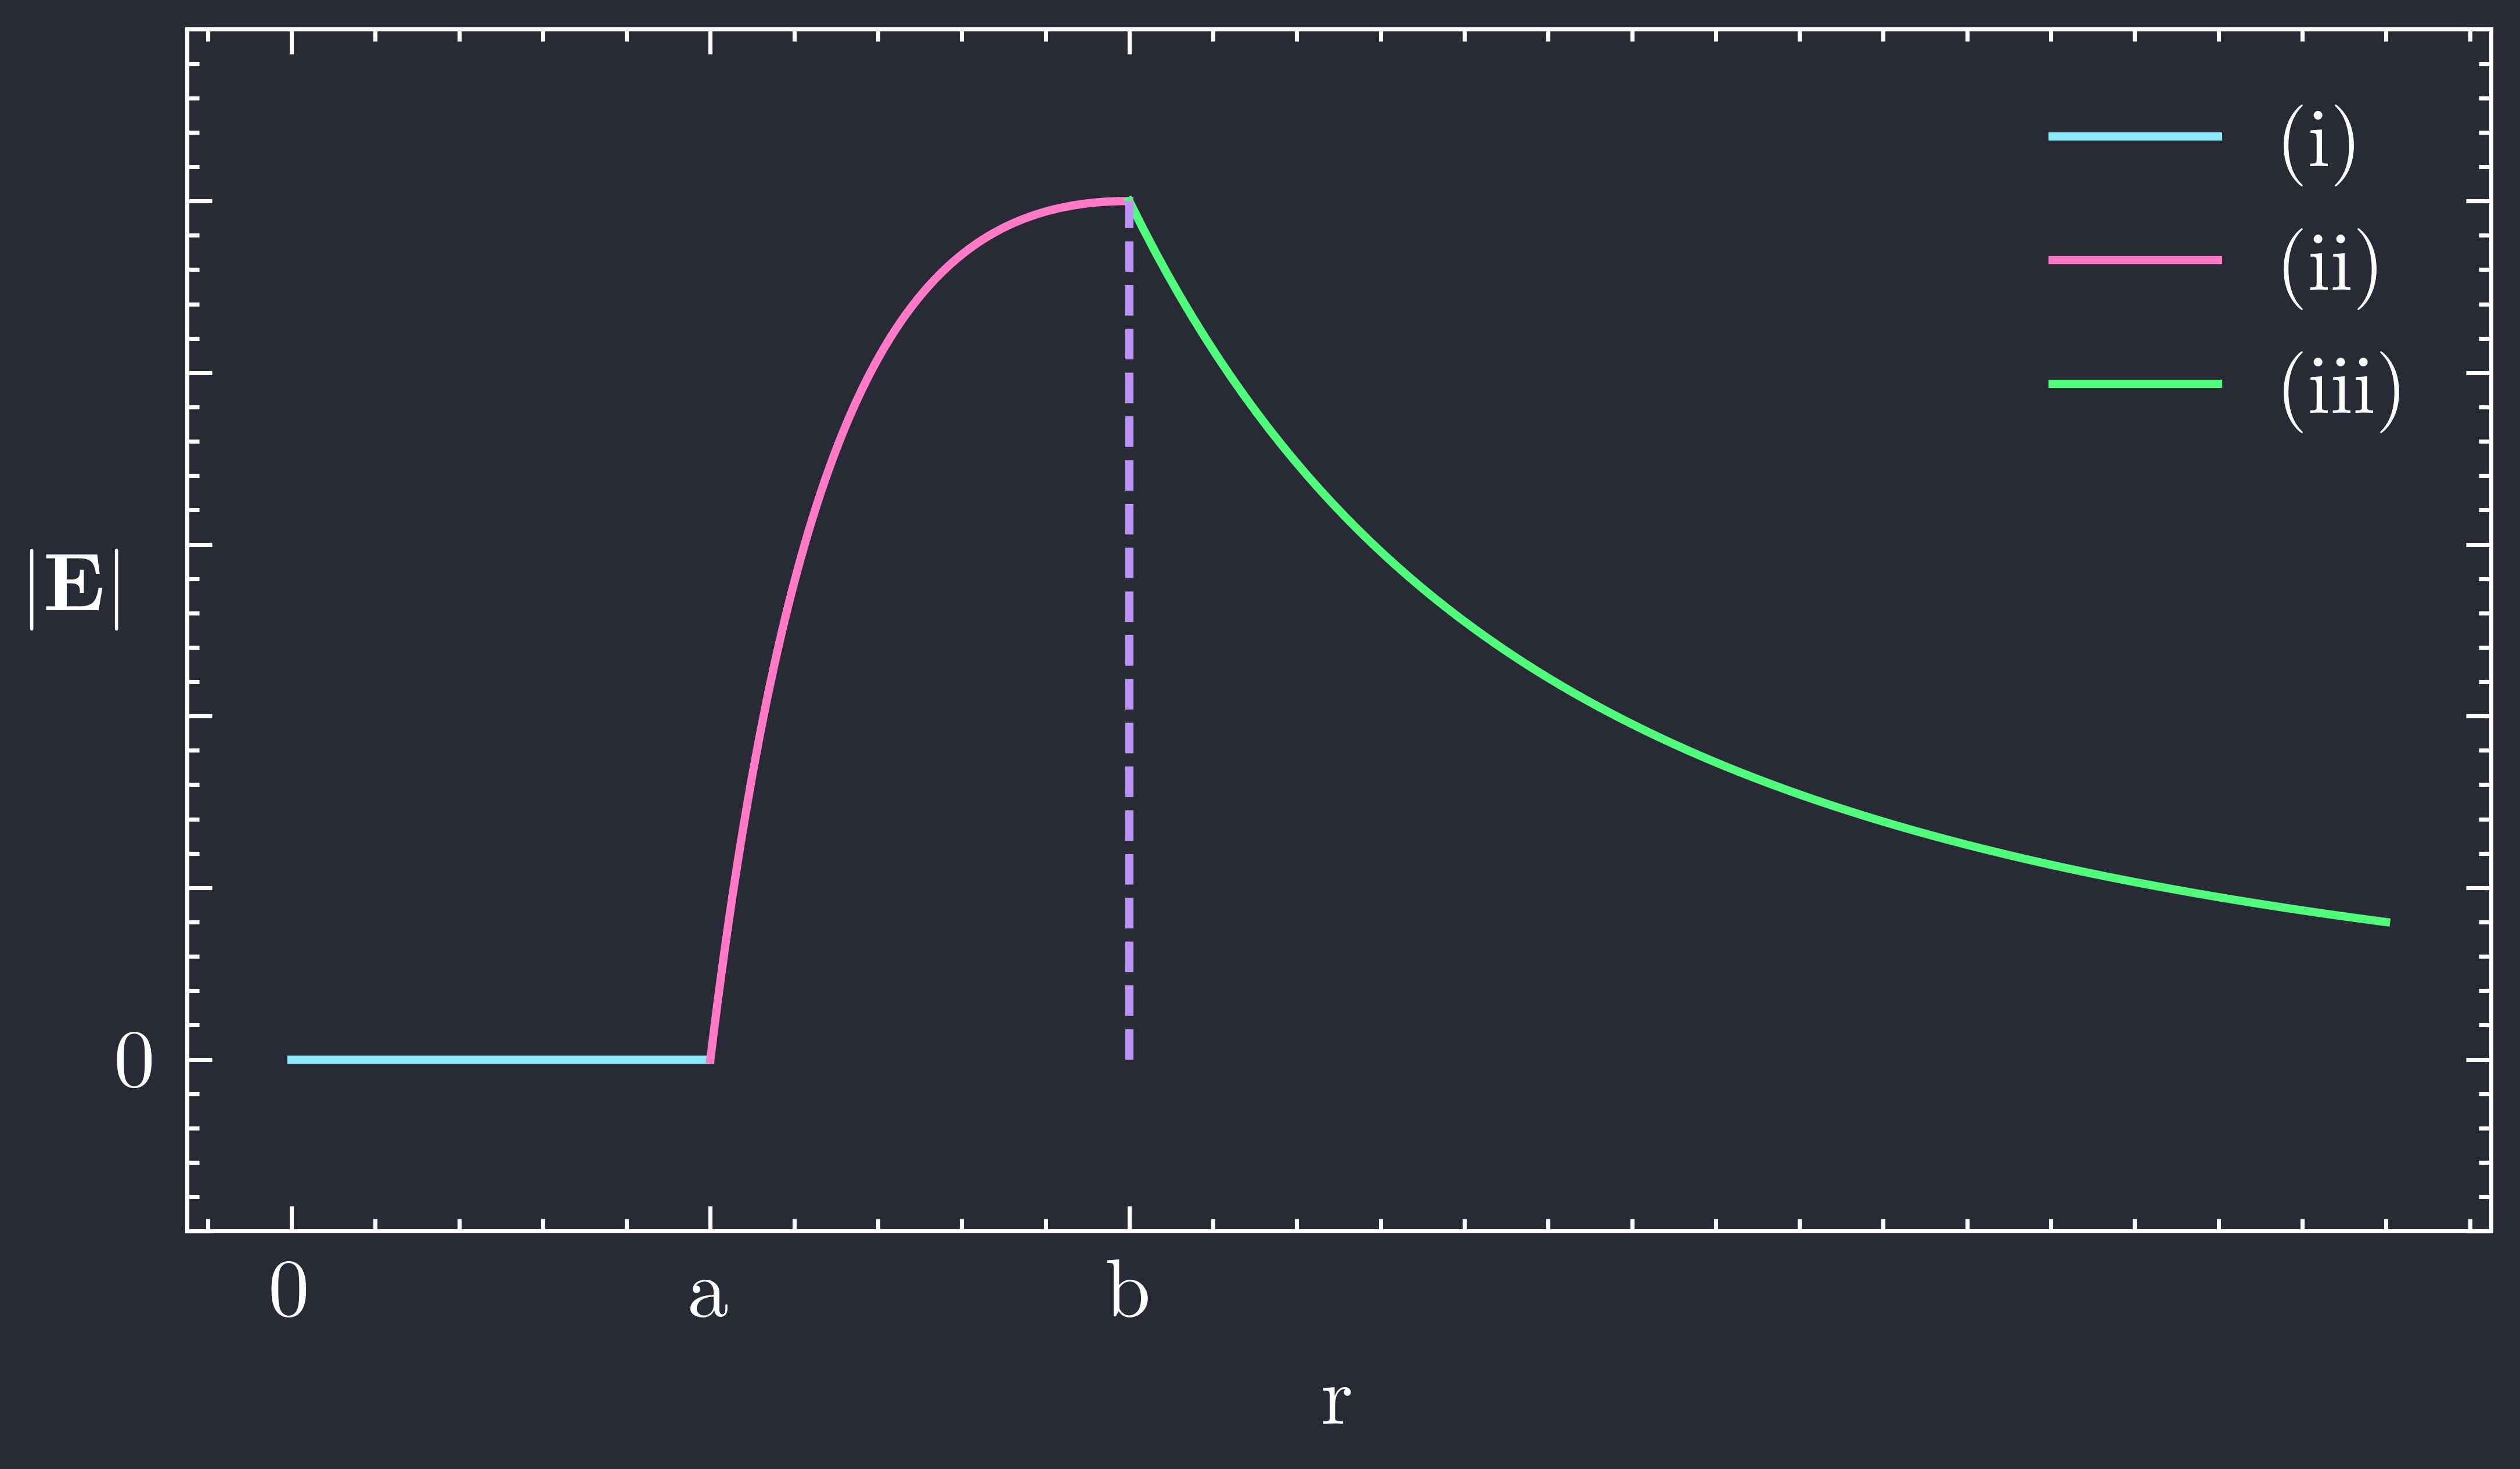
\includegraphics[width=0.5\linewidth]{images/fig2_15.png}
    \captionsetup{width=0.8\linewidth}
    \caption{Plot of $\abs{\vb{E}}$ as a function of $r$, for the case $b = 2a$.}
    \label{fig:2_15}
\end{figure}

\paragraph{2.16} \label{prob:2_16}
A long coaxial cable carries a uniform \emph{volume} charge charge density $\rho$ on the inner
cylinder (radius $a$), and a uniform \emph{surface} charge density $\sigma$ on the outer cylindrical
shell (radius $b$). This surface charge is negative, and the cable as a whole is electrically
neutral. Find the electric field in the three regions:

(i) Inside the inner cylinder \(r < a\): The enclosed charge is
\begin{align*}
    Q_{enc} = \rho \pi s^2 l
\end{align*}
where l is the length of the Gaussian cylinder. Using Gauss's law,
\begin{align*}
    \oint \vb{E} \vdot \dd{\vb{a}} &= \frac{1}{\epsilon_o} Q_{enc} \\
    \abs{\vb{E}} \int \dd{a} &= \frac{1}{\epsilon_o} \rho \pi s^2l \\
    E (2\pi sl) &= \frac{1}{\epsilon_o} \rho \pi s^2l \\
    \vb{E} = \frac{\rho s}{2\epsilon_o} \vu{s}
\end{align*}

(ii) Between the cylinders \(a \leq r \leq b\): The enclosed charge is
\[ Q_{enc} = \rho \pi a^2 l \]
thus the electric field is
\begin{align*}
    E (2\pi sl) &= \frac{1}{\epsilon_o} \rho \pi a^2 l \\
    \vb{E} = \frac{\rho a^2}{2\epsilon_o s} \vu{s}
\end{align*}

(iii) Outside the cable \(r > b\): The enclosed charge is
\[ Q_{enc} = \rho \pi a^2 l - \sigma \pi b l  = 0\]
thus the electric field is
\( \vb{E} = 0 \)

\begin{figure}[ht]
    \centering
    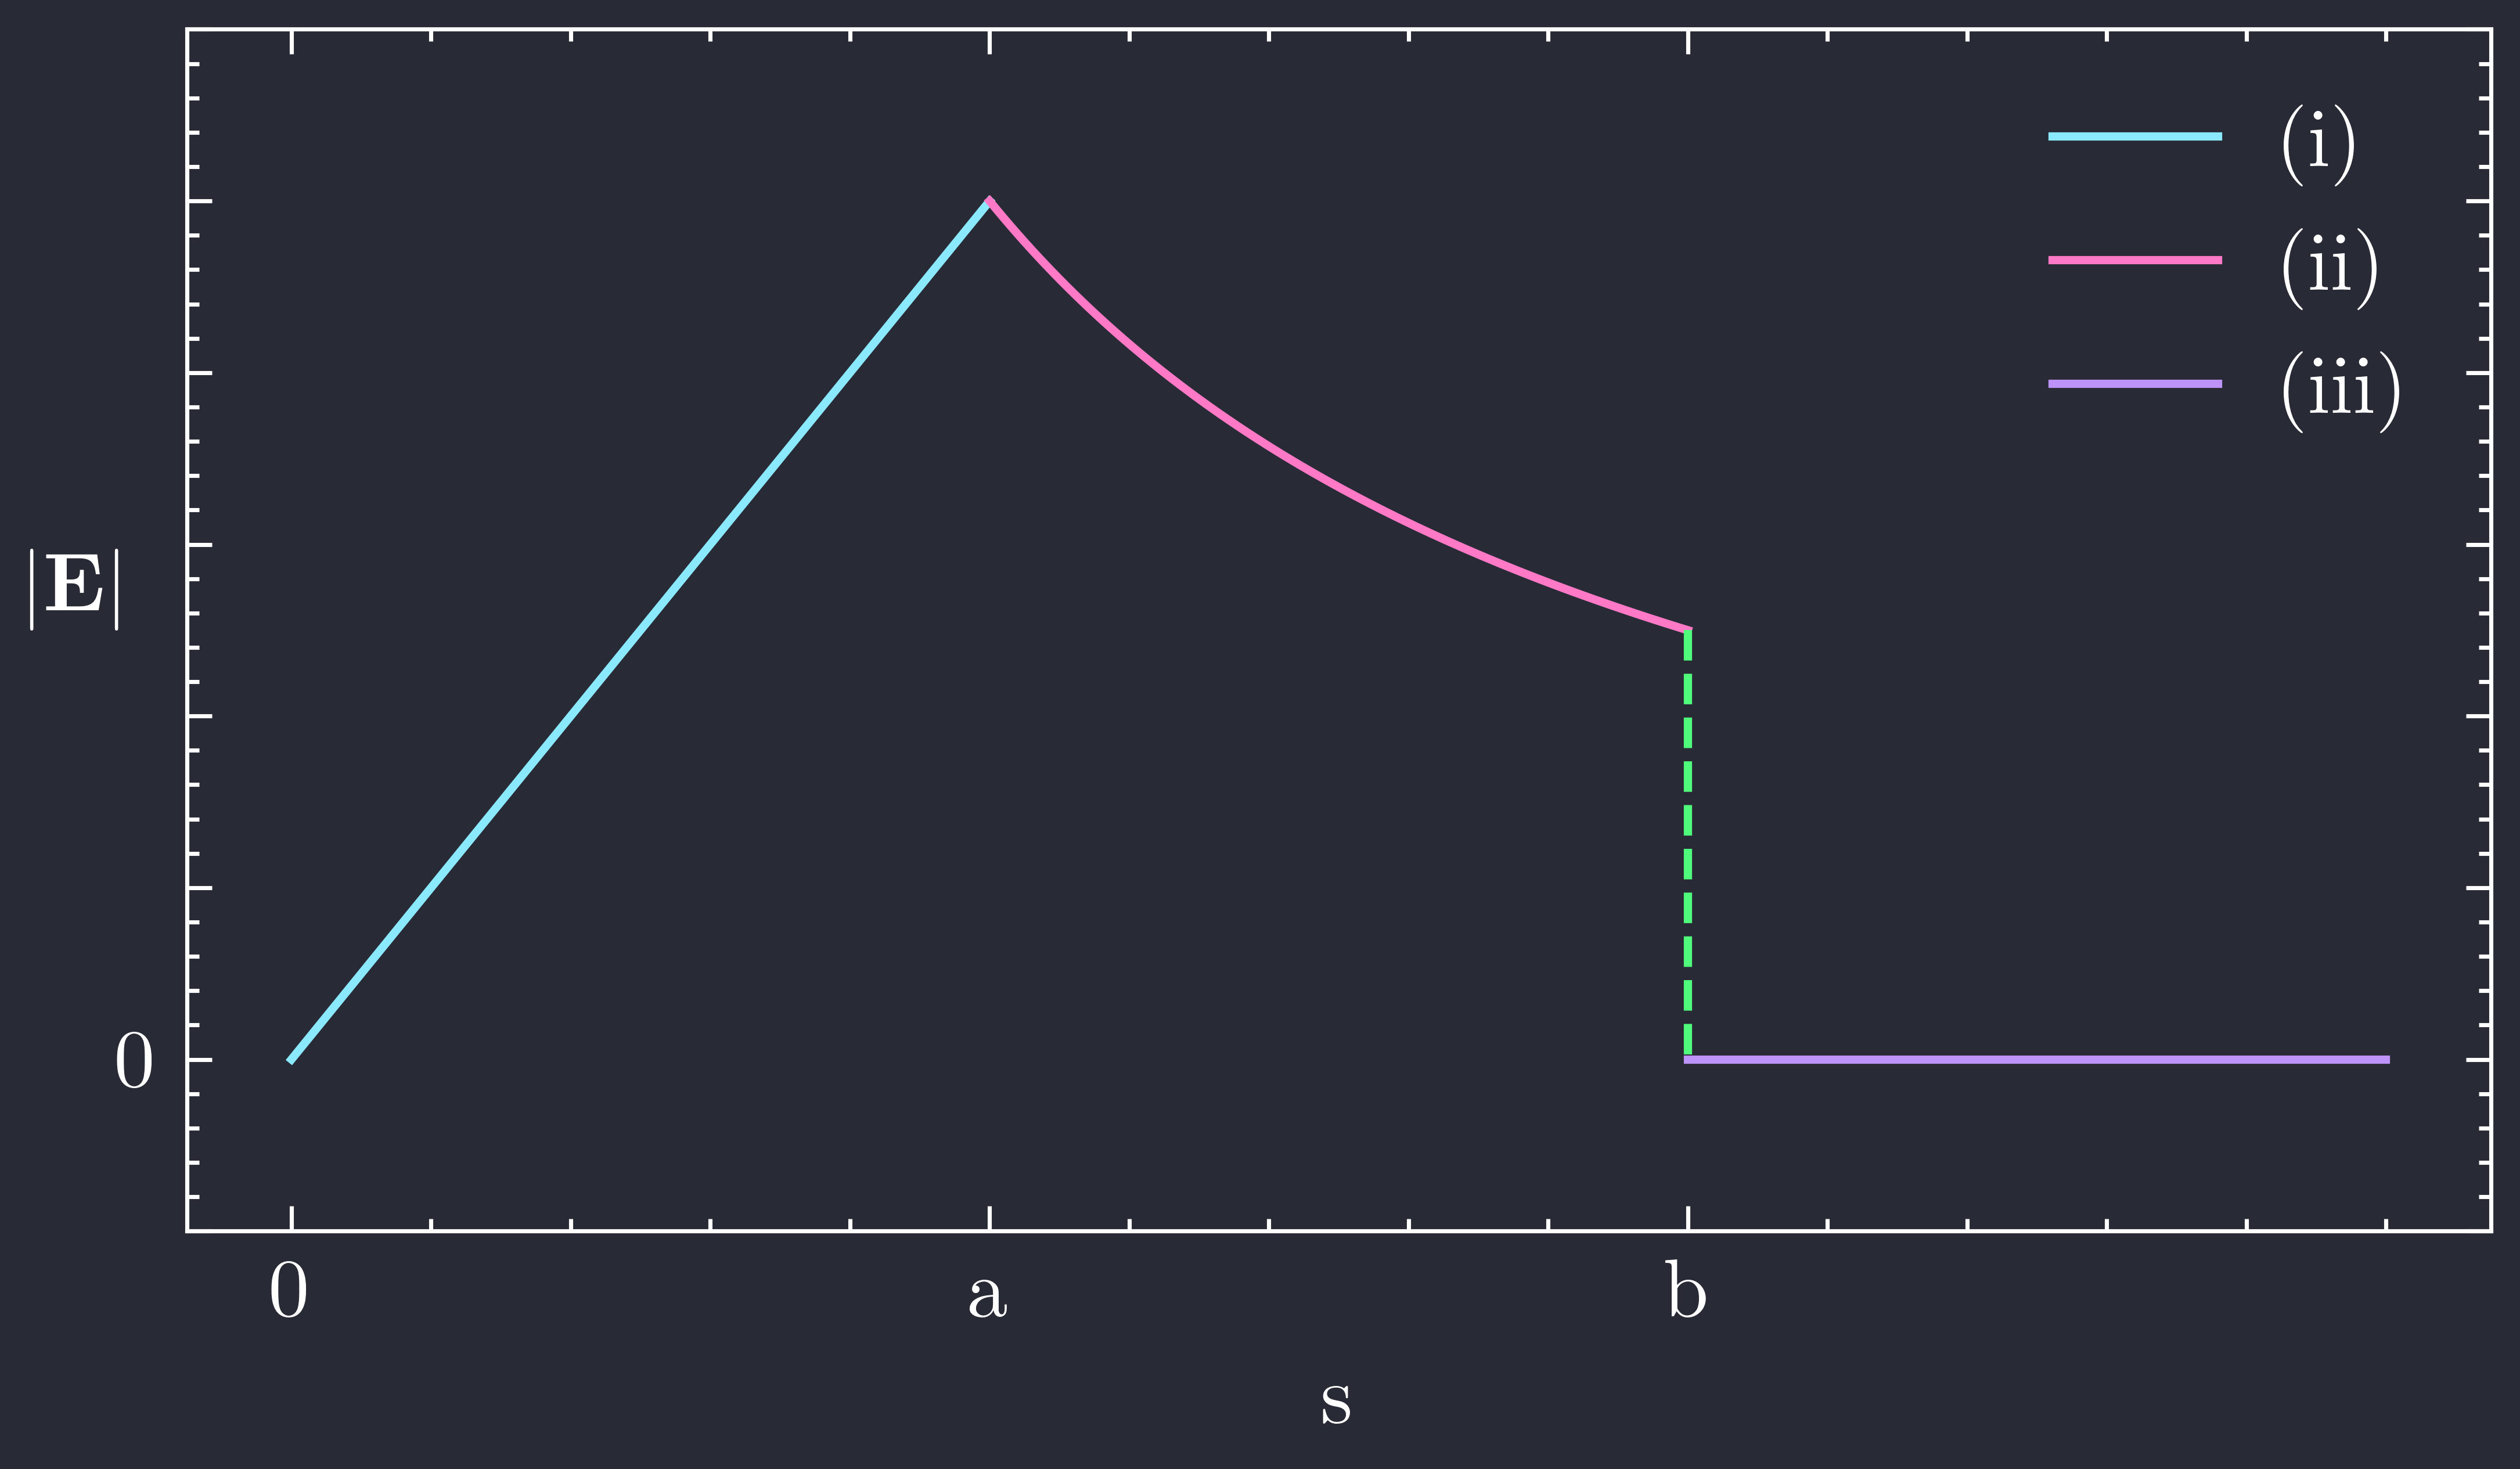
\includegraphics[width=0.5\linewidth]{images/fig2_16.png}
    \captionsetup{width=0.8\linewidth}
    \caption{Plot of $\abs{\vb{E}}$ as a function of $r$, for the case $b = 2a$.}
    \label{fig:2_16}
\end{figure}

\paragraph{2.17}
Finding the electric field, as a function of $y$, where $y=0$ is the center of an infinite plane
slab, of thickness $2d$, carrying a uniform volume charge density $\rho$. For the case \(y > 2d\)
The enclosed charge is
\begin{align*}
    Q_{enc} = \rho (2d) A = 2\rho Ad
\end{align*}
where $A$ is the area of the Gaussian pillbox. Using Gauss's law,
\begin{align*}
    \oint \vb{E} \vdot \dd{\vb{a}} &= \frac{1}{\epsilon_o} Q_{enc} \\
    \abs{\vb{E}} \int \dd{a} &= \frac{1}{\epsilon_o} 2\rho Ad \\
    E (2A) &= \frac{1}{\epsilon_o} 2\rho Ad \\
    \vb{E} &= \frac{\rho d}{\epsilon_o} \vu{y}
\end{align*}
For the case \(0 < y < 2d\), the enclosed charge is
\begin{align*}
    Q_{enc} = 2\rho y A
\end{align*}
and the electric field is
\begin{align*}
    E (2A) &= \frac{1}{\epsilon_o} \rho y A \\
    \vb{E} &= \frac{\rho y}{\epsilon_o} \vu{y}
\end{align*}
In the $-y$ direction, $E$ is negative as shown in Figure \ref{fig:2_17}.
\begin{figure}
    \centering
    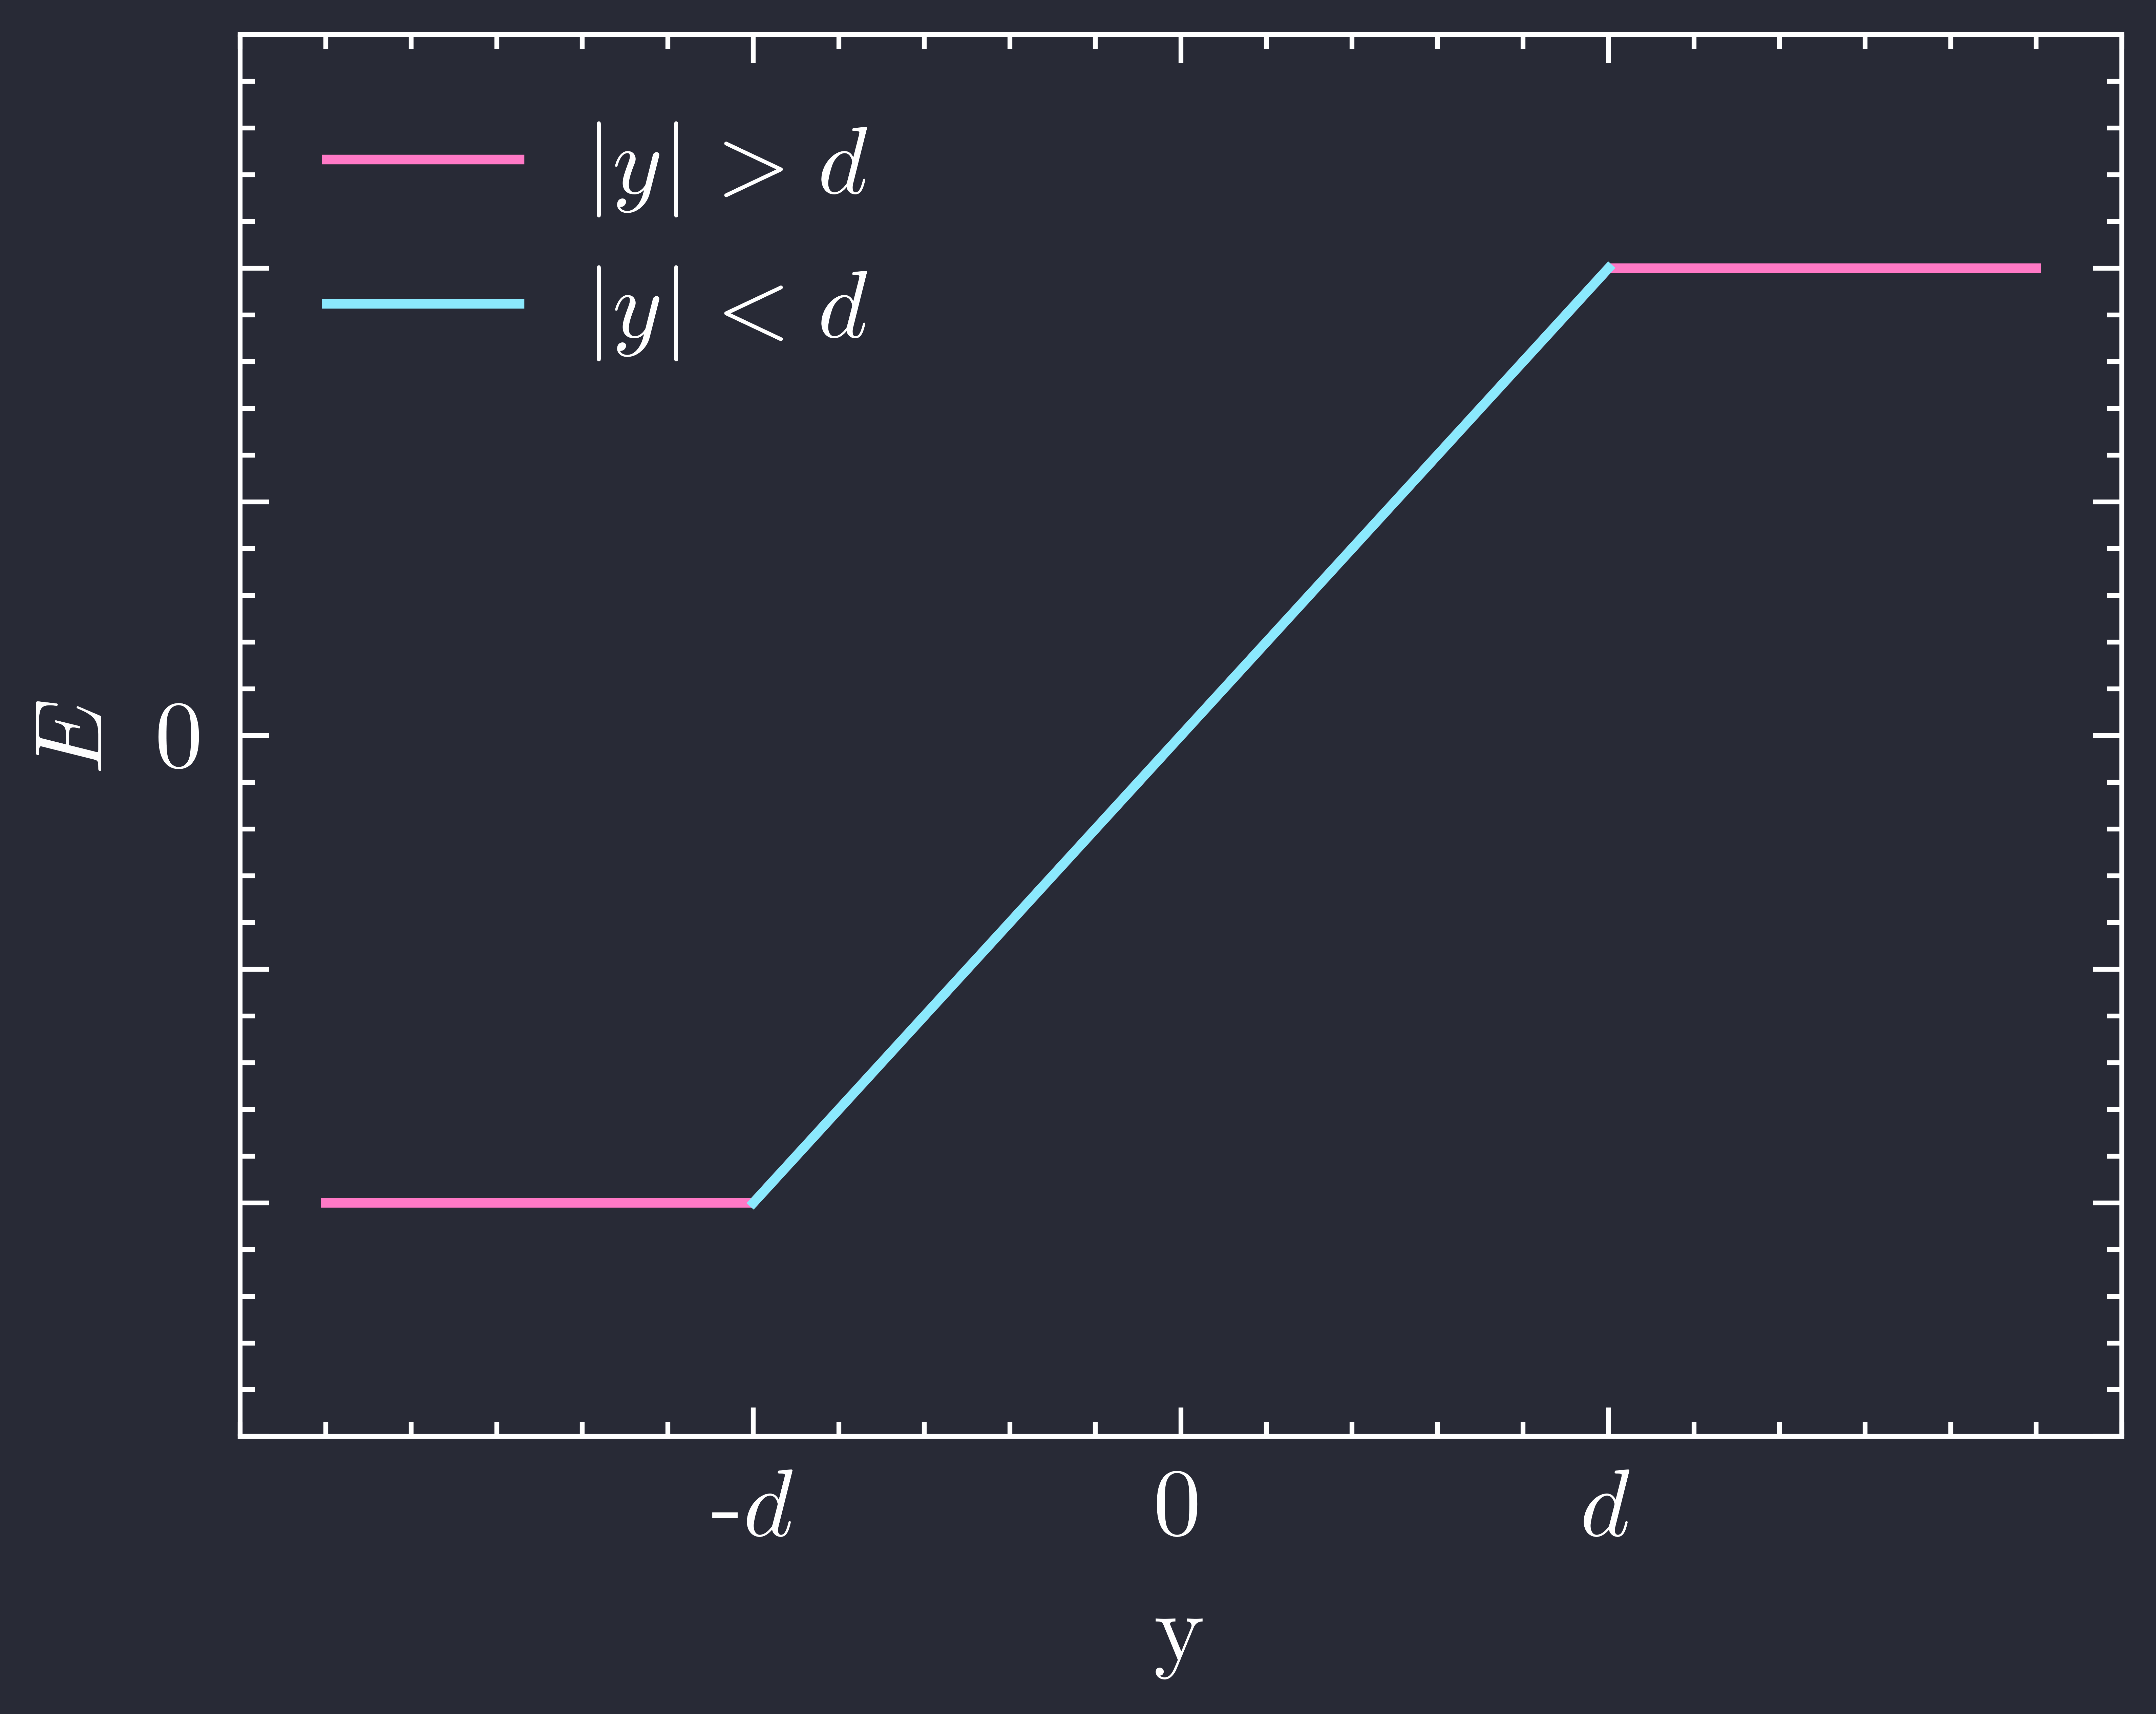
\includegraphics[width=0.5\linewidth]{images/fig2_17.png}
    \captionsetup{width=0.8\linewidth}
    \caption{Plot of $\abs{\vb{E}}$ as a function of $y$}
    \label{fig:2_17}
\end{figure}

\paragraph{2.18}
For two spheres of radius $R$ and charge density $+\rho$ and $-\rho$, respectively, are partially
overlapping. From Prob 2.12, the electric field inside a sphere of radius $R$ with a uniform volume
charge density $\rho$ is
\[ \vb{E} = \frac{1}{3\epsilon_o} \rho \vb{r} \]
where $\vb{r}$ is the position vector from the center of the sphere. The electric field for each 
sphere is
\begin{align*}
    \vb{E}_1 &= \frac{1}{3\epsilon_o} \rho \vb{r}_1 \\
    \vb{E}_2 &= -\frac{1}{3\epsilon_o} \rho \vb{r}_2
\end{align*}
Thus the total electric field is
\begin{align*}
    \vb{E} &= \frac{1}{3\epsilon_o} \rho (\vb{r}_1 - \vb{r}_2) \\
    &= \frac{1}{3\epsilon_o} \rho \vb{d}
\end{align*}
where $\vb{d}$ is the vector from the positive center to the negative center. Thus the electric
field is constant inside the overlapping region.

\paragraph{2.19}
The electric field inside a sphere of radius $R$ with a uniform volume charge density $\rho$ is
\[\tag{2.8} \label{eq:2_8}
    \vb{E}(r) = \ke \int \frac{\hat \boldscriptr}{\scriptr^2} \rho(\vb{r}') \dd{\tau'}
\]
The curl of \eqref{eq:2_8} is
\[
    \curl \vb{E} = \ke \int \curl \qt(\frac{\hat \boldscriptr}{\scriptr^2}) \rho(\vb{r}') \dd{\tau'}
\]
From Prob 1.63, \( \curl \frac{\hat \boldscriptr}{\scriptr^2} = 0 \), thus
\[ \curl \vb{E} = 0 \]

\paragraph{2.20}
From the conservative nature of the electric field, the curl of the electric field is zero:
(a) \( \vb{E} = k[xy \vu{x} + 2yz \vu{y} + 3xz \vu{z}] \);
\[
    \curl{\vb{E}}_a = k \begin{vmatrix}
        \vu{x} & \vu{y} & \vu{z} \\
        \pdv{x} & \pdv{y} & \pdv{z} \\
    xy & 2yz & 3xz
    \end{vmatrix}
    = k [-2y \vu{x} - 3z \vu{y} - x \vu{z}] \neq 0
\]
Thus (a) is not a possible electric field. \\
(b) \( \vb{E}_b = k[y^2 \vu{x} + (2xy + z^2) \vu{y} + 2yz \vu{z}] \);
\[
    \curl \vb{E}_b = k \begin{vmatrix}
        \vu{x} & \vu{y} & \vu{z} \\
        \pdv{x} & \pdv{y} & \pdv{z} \\
        y^2 & 2xy + z^2 & 2yz    
    \end{vmatrix}
    = 0
\]
So (b) is a possible electric field. Finding a potential using the origin as the reference point:
\[ \tag{2.21} \label{eq:2_21}
    V = - \int_O^{\vb{r}} \vb{E} \vdot \dd{\vb{l}}
\]
Setting the path of integration into three parts: \\
(I) From $O \to A = (x,0, 0)$;
\[
    \dd{\vb{l}} = \dd{x} \vu{x}; \quad \vb{E} \vdot \dd{\vb{l}} = ky^2 \dd{x} = 0; \quad
    \int_O^A \vb{E} \vdot \dd{\vb{l}} = 0
\]
(II) From $A \to B = (x,y,0)$;
\[
    \dd{\vb{l}} = \dd{y} \vu{y}; \quad \vb{E} \vdot \dd{\vb{l}} = k(2xy + z^2) \dd{y} = 2kxy \dd{y};
    \quad \int_A^B \vb{E} \vdot \dd{\vb{l}} = 2kx \int_0^y y' \dd{y'} = kxy^2
\]
(III) From $B \to C = (x,y,z)$;
\[
    \dd{\vb{l}} = \dd{z} \vu{z}; \quad \vb{E} \vdot \dd{\vb{l}} = 2kyz; \quad
    \int_B^C \vb{E} \vdot \dd{\vb{l}} = 2ky \int_0^z z' \dd{z'} = kyz^2
\]
So the potential is
\begin{align*}
    V = - \qt( \int_O^A \vb{E} \vdot \dd{\vb{l}} + \int_A^B \vb{E} \vdot \dd{\vb{l}}
        + \int_B^C \vb{E} \vdot \dd{\vb{l}} ) = -k(xy^2 + yz^2)
\end{align*}
Checking the potential function using the gradient:
\[
    -\grad V = k(y^2 \vu{x} + (2xy + z^2) \vu{y} + 2yz \vu{z}) = \vb{E}_b
\]

\paragraph{2.21} \label{prob:2_21}
Find the potential inside and outside a uniformly charged solid sphere whose radius is $R$ and whose
total charge is $q$. Use infinity as your reference point. Compute the gradient of $V$ in each
region, and check that it yields the correct field. Sketch $V(r)$.
\barh
The electric field outside the sphere is
\[ \vb{E}_{out} = \ke \frac{q}{r^2} \vu{r} \]
and from Problem \nameref{prob:2_8}, the electric field inside the sphere is
\[ \vb{E}_{in} = \ke \frac{q}{R^3} r \vu{r} \]
For points outside the sphere $(r > R)$,
\[
    V(r) = - \int_\infty^r \vb{E} \vdot \dd{\vb{l}} = - \ke \int_\infty^r \frac{q}{r'^2} \vu{r}
    = \ke \frac{q}{r'} \eval_\infty^r = \ke \frac{q}{r}
\]
For points inside the sphere $(r < R)$,
\begin{align*}
    V(r) &= - \int_\infty^R \vb{E} \vdot \dd{\vb{l}} - \int_R^r \vb{E} \vdot \dd{\vb{l}} \\
    &= \ke \frac{q}{R} - \ke \frac{q}{R^2} \int_R^r r' \dd{r'} \\
    &= \ke \frac{q}{R} - \ke \frac{q}{R^2} \qt(\frac{r'^2}{2}) \eval_R^r \\
    &= \ke \frac{q}{2R} \qt(3 - \frac{r^2}{R^2}) 
\end{align*}
The gradient of $V$ for $r > R$:
\[ -\grad V = \ke \frac{q}{r^2} \vu{r} = \vb{E}_{out} \]
and for $r < R$:
\[ -\grad V = \ke \frac{q}{R^3} r \vu{r} = \vb{E}_{in} \]
\begin{figure}[ht]
    \centering
    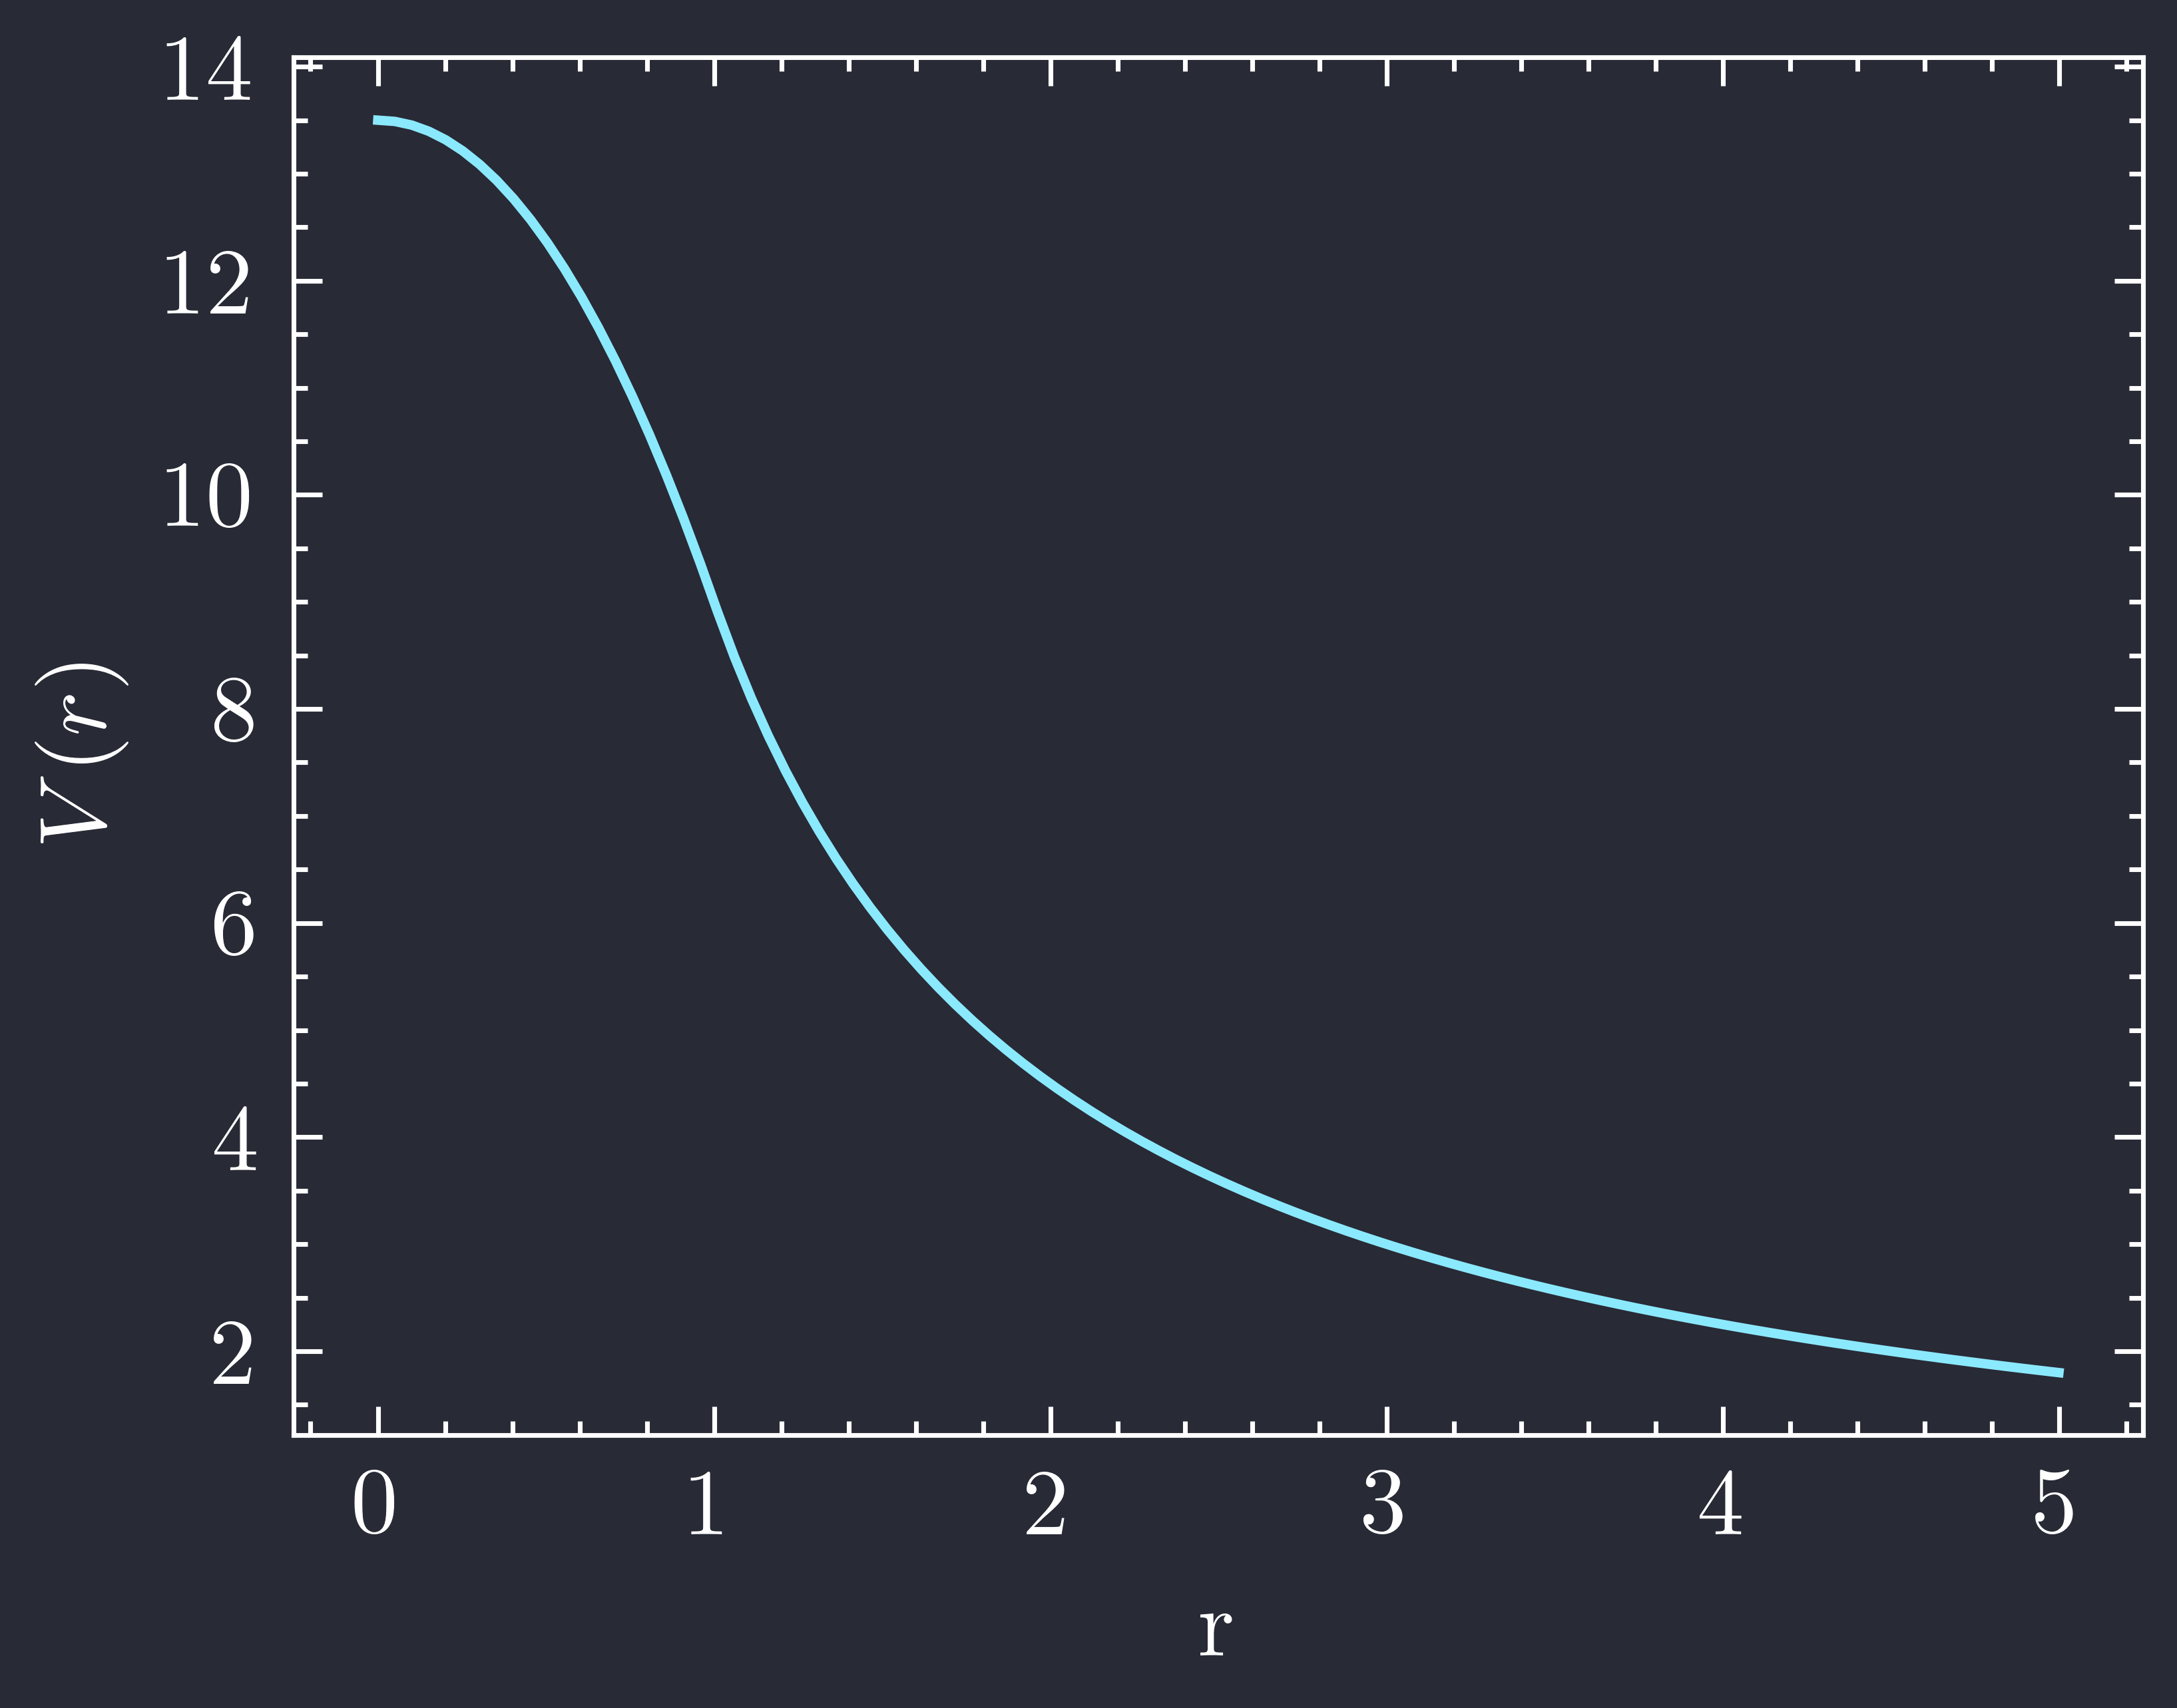
\includegraphics[width=0.5\linewidth]{images/fig2_21.png}
    \captionsetup{width=0.8\linewidth}
    \caption{Plot of $V(r)$ as a function of $r$ where $q = \qty{1}{nC}$ and $R = \qty{1}{m}$.}
    \label{fig:2_21}
\end{figure}

\paragraph{2.22} \label{prob:2_22}
From Problem \nameref{prob:2_13}, the electric field a distance $s$ from an infinitely long straight
wire is
\[ \vb{E} = \ke \frac{2\lambda}{s} \vu{s} \]
where $\lambda$ is the linear charge density of the wire. Setting the reference point at an
arbitrary point $s_0$,
\begin{align*}
    V(s) &= - \int_{s_0}^s \vb{E} \vdot \dd{\vb{l}} \\
    &= - \ke \int_{s_0}^s \frac{2\lambda}{s'} \dd{s'} \\
    &= - \ke 2\lambda \ln(\frac{s}{s_0})
\end{align*}
And the gradient of $V$ is
\begin{align*}
    -\grad V &= \ke \frac{2\lambda}{s} \vu{s} = \vb{E}
\end{align*}

\paragraph{2.23}
From Problem \nameref{prob:2_15}, the electric field in the three regions are:
\begin{enumerate}
    \item[(i)] Inside the inner sphere, $r < a$:
    \[ \vb{E}_1 = 0 \]
    \item[(ii)] Between the spheres, $a \leq r \leq b$:
    \[ \vb{E}_2 = \frac{k(r - a)}{\epsilon_o r^2} \vu{r} \]
    \item[(iii)] Outside the outer sphere, $r > b$:
    \[ \vb{E}_3 = \frac{k(b - a)}{\epsilon_o r^2} \vu{r} \]
\end{enumerate}
To find the potential at the center, the reference point is set to $\infty$, and the line element is
$\dd{\vb{l}} = \dd{r} \vu{r}$:
\begin{align*}
    V(r) &= - \int_\infty^O \vb{E} \vdot \dd{\vb{l}} \\
    &= - \int_\infty^b \vb{E}_3 \vdot \dd{\vb{l}} - \int_b^a \vb{E}_2 \vdot \dd{\vb{l}}
        - \int_a^0 \vb{E}_1 \vdot \dd{\vb{l}} \\
    &= - \int_\infty^b \frac{k(b - a)}{\epsilon_o r^2} \dd{r}
        - \int_b^a \frac{k(r - a)}{\epsilon_o r^2} \dd{r} - \int_a^0 0 \dd{r} \\
    &= \frac{k}{\epsilon_o} \frac{b - a}{b}
        - \frac{k}{\epsilon_o} \qt(\ln(\frac{a}{b}) + 1 - \frac{a}{b}) \\
    &= - \frac{k}{\epsilon_o} \ln(\frac{a}{b})
\end{align*}

\paragraph{2.24}
From Problem \nameref{prob:2_16}, the potential difference betwen a point on the axis $(s = 0)$ and
a point on the outside cylinder $(s = b)$ goes through two distinct electric fields:
\begin{enumerate}
    \item[(i)] Inside the inner cylinder, $s < a$:
    \[ \vb{E}_1 = \frac{\rho s}{2\epsilon_o} \vu{s} \]
    \item[(ii)] Between the cylinders, $a \leq s \leq b$:
    \[ \vb{E}_2 = \frac{\rho a^2}{2\epsilon_o s} \vu{s} \]
\end{enumerate}
So the potential difference is (using the line element $\dd{\vb{l}} = \dd{s} \vu{s}$):
\begin{align*}
    V(b) - V(0) &= - \int_0^b \vb{E} \vdot \dd{\vb{l}} \\
    &= - \int_0^a \vb{E}_1 \vdot \dd{\vb{l}} - \int_a^b \vb{E}_2 \vdot \dd{\vb{l}} \\
    &= - \int_0^a \frac{\rho s}{2\epsilon_o} \dd{s}
    - \int_a^b \frac{\rho a^2}{2\epsilon_o s} \dd{s} \\
    &= - \frac{\rho}{2\epsilon_0} \qt(\int_0^a s \dd{s} + a^2 \int_a^b \frac{1}{s} \dd{s}) \\
    &= - \frac{\rho}{2\epsilon_o} \qt(\frac{a^2}{2} + a^2 \ln(\frac{b}{a})) \\
    &= - \frac{\rho a^2}{4\epsilon_o} \qt(1 + 2\ln(\frac{b}{a}))
\end{align*}

\paragraph{2.25} \label{prob:2_25}
From Griffiths % griffiths 2.27 + 2.30
\begin{align*} \tag{2.27} \label{eq:2_27}
    V(r) &= \ke \sum_{i = 1}^n \frac{q_i}{\scriptr_i}
\end{align*}
and
\begin{align*} \tag{2.30} \label{eq:2_30}
    V = \ke \int \frac{\lambda(\vb r')}{\scriptr} \dd{\ell'} \qand V = \ke \int \frac{\sigma(\vb r')}{\scriptr} \dd{a'} 
\end{align*}
\begin{enumerate}
    \item [(a.1)] Two point charges $+q$ a distance $d$ apart: Find the potential a distance $z$ above the center of the charges:
    \begin{figure*}[ht]
        \centering
        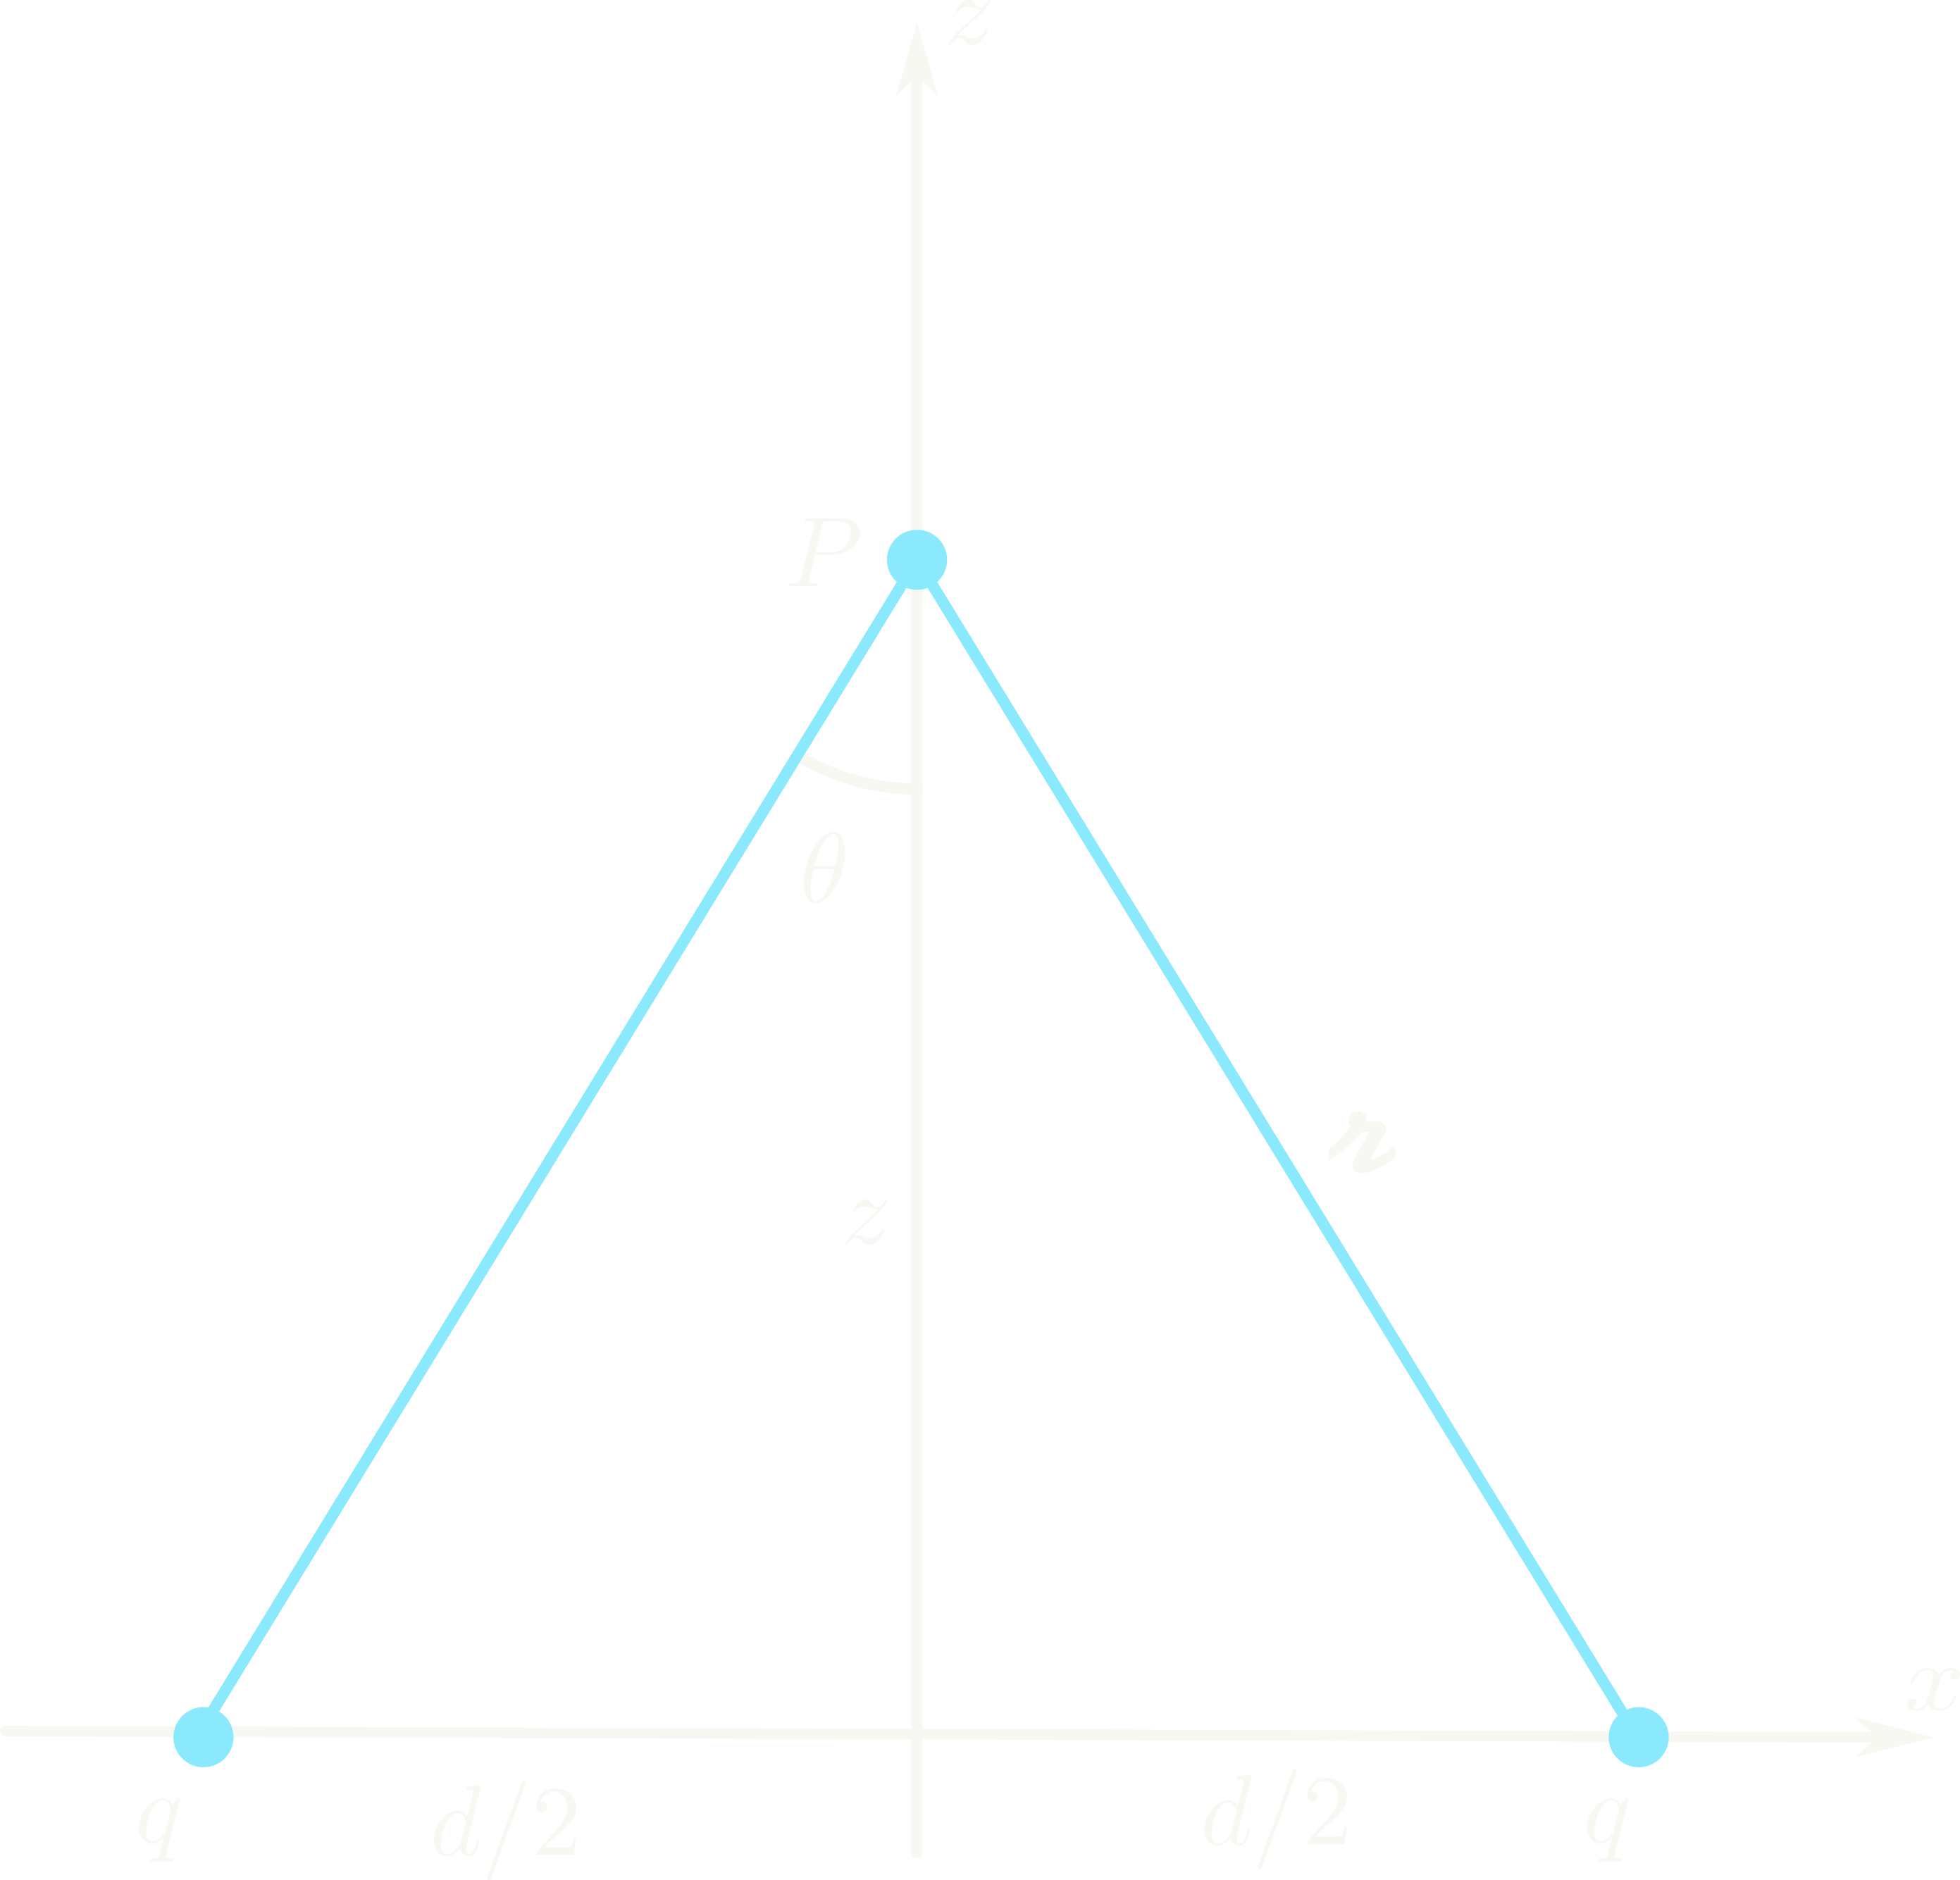
\includegraphics[width=0.5\linewidth]{images/hw2_25a.png}
        \captionsetup{width=0.8\linewidth}
        \caption{Two point charges $+q$ a distance $d$ apart.}
        \label{fig:2_25a}
    \end{figure*}
    Using Eq. \eqref{eq:2_27}, the potential is
    \begin{align*}
        &V_a = \ke \qt(\frac{q}{\sqrt{z^2 + \frac{d^2}{4}}} + \frac{q}{\sqrt{z^2 + \frac{d^2}{4}}}) \\
        &\boxed{V_a = \ke \frac{2q}{\sqrt{z^2 + \frac{d^2}{4}}}}
    \end{align*}
    \item [(a.2)] Computing the electric field $\vb E = -\grad V$:
    \begin{align*}
        \vb E_a &= -\pdv{V_a}{z} \vu z \\
        &= -\ke \frac{-1}{2} \frac{2q(2z)}{\qt(z^2 + \frac{d^2}{4})^{3/2}} \vu z
    \end{align*}
    simplifying to
    \begin{align*}
        \boxed{\vb E_a = \ke \frac{2qz}{\qt(z^2 + \frac{d^2}{4})^{3/2}} \vu z}
    \end{align*}
    which is the same as Ex. 2.1
    \begin{figure*}
        \centering
        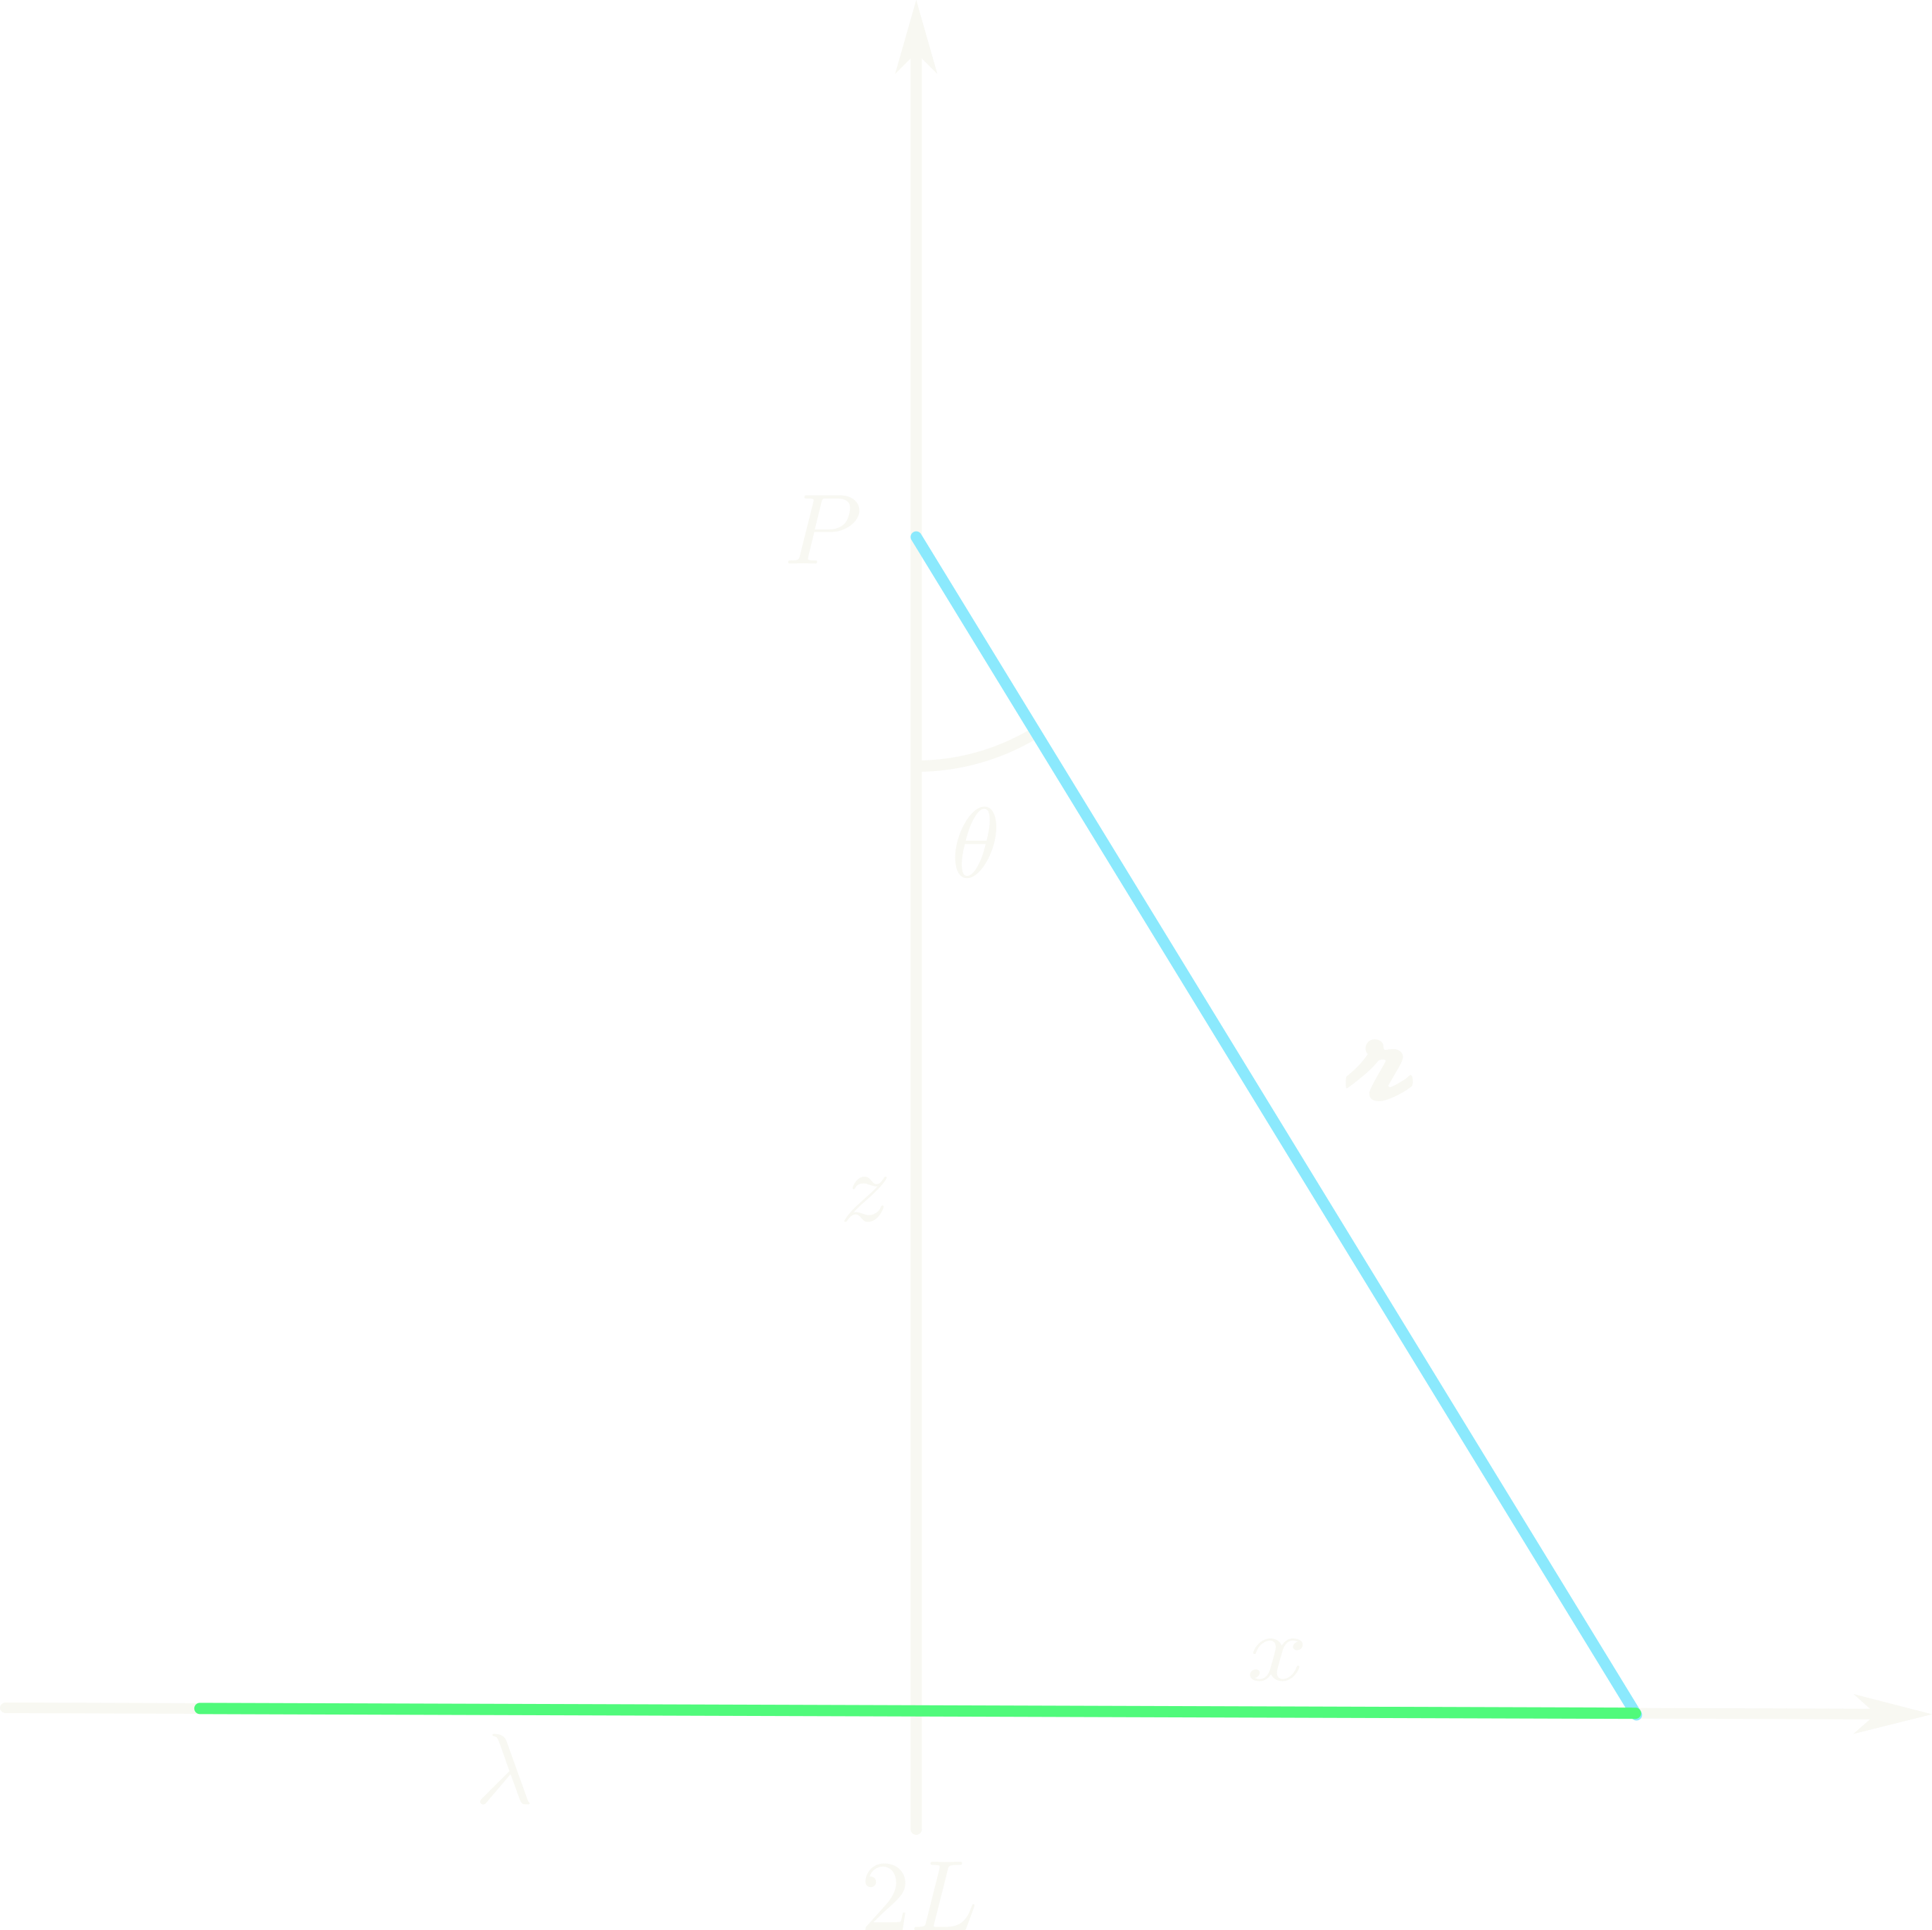
\includegraphics[width=0.5\linewidth]{images/hw2_25b.png}
        \captionsetup{width=0.8\linewidth}
        \caption{A line charge of density $\lambda$.}
        \label{fig:2_25b}
    \end{figure*}
    \item [(b.1)] Using Eq. \eqref{eq:2_30}, the potential is
    \begin{align*}
        V_b &= \ke \lambda \int_{-L}^L \frac{1}{\sqrt{z^2 + x^2}} \dd{x}
    \end{align*}
    To solve the integral, we can use the substitution from the trig identity
    \begin{align*}
        \cosh^2 u - \sinh^2 u &= 1 \\
        \implies z^2 \cosh^2 u &= z^2 + z^2\sinh^2 u \\
        &= z^2 + x^2
    \end{align*}
    where 
    \begin{align*}
        x &= z \sinh u \implies u = \arcsinh \frac{x}{z} \\
        \dd{x} &= z \cosh u \dd{u}
    \end{align*}
    Thus the integral becomes
    \begin{align*}
        V_b &= \ke \lambda \int \frac{\cancel{z \cosh u}}{\cancel{z \cosh u}} \dd{u} \\
        &= \ke \lambda u \eval_{-L}^L \\
        &= \ke \lambda \qt[\arcsinh{\frac{L}{z}} - \arcsinh{\frac{-L}{z}}]
    \end{align*}
    Using $\arcsinh \qt(a) = \ln \abs{a + \sqrt{a^2 + 1}}$:
    \begin{align*}
        \implies \arcsinh(\frac{L}{z}) &= \ln \abs{\frac{L}{z} + \sqrt{\qt(\frac{L}{z})^2 + 1}} \\
        &= \ln \abs{\frac{1}{z}(L + \sqrt{L^2 + z^2})}
    \end{align*}
    so the potential is
    \begin{align*}
        \boxed{V_b = \ke \lambda \ln \abs{\frac{L + \sqrt{L^2 + z^2}}{-L + \sqrt{L^2 + z^2}}}}
    \end{align*}
    \item[(b.2)] The electric field is
    \begin{align*}
        \vb E_b &= -\pdv{V_b}{z} \vu z \\
        &= -\ke \lambda \qt[ \frac{1}{L + \sqrt{L^2 + z^2}} \qt(\frac{1}{2} \frac{2z}{\sqrt{L^2 + z^2}})
            - \frac{1}{-L + \sqrt{L^2 + z^2}} \qt(\frac{1}{2} \frac{2z}{\sqrt{L^2 + z^2}})]\vu z \\
        &= -\ke \lambda \frac{z}{\sqrt{L^2 + z^2}} \qt[\frac{-L + \sqrt{L^2 + z^2}}{-L^2 + (L^2 + z^2)} - \frac{L + \sqrt{L^2 + z^2}}{-L^2 + (L^2 + z^2)}] \vu z \\
        &= -\ke \lambda \frac{-2Lz}{z^2 \sqrt{L^2 + z^2}} \vu z
    \end{align*}
    simplifying to
    \begin{align*}
        \boxed{\vb E_b = \ke \frac{2\lambda L}{z \sqrt{L^2 + z^2}} \vu z}
    \end{align*}
    which is the same as Ex. 2.2

    \item[(c.1)] Using Eq. \eqref{eq:2_30} and polar coordinates, the potential is
    \begin{align*}
        V_c &= \ke \sigma \int_0^{2\pi} \int_0^R \frac{1}{\sqrt{z^2 + r^2}} r \dd{r} \dd{\theta} \\
        &= \ke 2\pi \sigma \int_0^R \frac{r}{\sqrt{z^2 + r^2}} \dd{r}
    \end{align*}
    substituting $u = z^2 + r^2$; $\dd{u} = 2r \dd{r}$:
    \begin{align*}
        V_c &= \ke \pi \sigma \int \frac{1}{\sqrt{u}} \dd{u} \\
        &= \ke \pi \sigma 2 \sqrt{z^2 + r^2} \eval_0^{R}
    \end{align*}
    thus
    \begin{align*}
        \boxed{V_c = \frac{\sigma}{2\epsilon_0} \qt[\sqrt{z^2 + R^2} - z]}
    \end{align*}
    \item[(c.2)] The electric field is
    \begin{align*}
        \vb E_c &= -\pdv{V_c}{z} \vu z \\
        &= -\frac{\sigma}{2\epsilon} \qt[\frac{z}{\sqrt{z^2 + R^2}} - 1] \vu z
    \end{align*}
    thus
    \begin{align*}
        \boxed{\vb E_c = \frac{\sigma}{2\epsilon_0} \qt[1 - \frac{z}{\sqrt{z^2 + R^2}}] \vu z}
    \end{align*}
    which is the same as Problem 2.6:
    \paragraph{2.6}
The electric field is only in the $z$-direction where $\cos\theta = z/\scriptr$:
\begin{align*}
    \vb{E} &= \frac{1}{4\pi\epsilon_0}
        \int \frac{\sigma}{\scriptr^2} \cos\theta \vu{z} \dd{\vb{a}} \\
    &= \frac{1}{4\pi\epsilon_0}
        \int \frac{\sigma z}{(z^2 + r^2)^{3/2}} \vu{z} \dd{\vb{a}}
\end{align*}
Using polar coordinates: since $\dd{\vb{a}} = r \dd{r} \dd{\theta} $
\begin{align*}
    \vb{E} &= \frac{1}{4\pi\epsilon_0}
        \int_0^{2\pi} \int_0^R \frac{\sigma z}{(z^2 + r^2)^{3/2}} \vu{z} r \dd{r} \dd{\theta} \\
    &= \frac{1}{4\pi\epsilon_0}
        \sigma z (2\pi) \vu{z} \int_0^R \frac{r}{(z^2 + r^2)^{3/2}} \dd{r} \\
    &= \frac{\sigma}{2\epsilon_0} z \vu{z} \qt[
            -\frac{1}{\sqrt{z^2 + r^2}}
        ]_0^R \\
    &= \frac{\sigma}{2\epsilon_0} z  \qt[
            \frac{1}{z} -\frac{1}{\sqrt{z^2 + R^2}}
        ] \vu{z} \\
    \vb E &= \frac{\sigma}{2\epsilon_0} \qt[1 - \frac{1}{\sqrt{z^2 + R^2}}] \vu{z}
\end{align*}
    \item[(d)] if the right-hand charge of Fig. \ref{fig:2_25a} is replaced by a charge $-q$, the potential at $P$ using Eq. \eqref{eq:2_27} is
    \begin{align*}
        V_d = 0 \implies \vb E_d = 0
    \end{align*}
    which contradicts the result from Prob 2.2. This is because point $P$ does not give us any information about the electric field which points in the $x$-direction.
    In fact any reference point on the $z$-axis will give us the same result. 
\end{enumerate}

\paragraph{2.26}
\begin{figure}[ht]
    \centering
    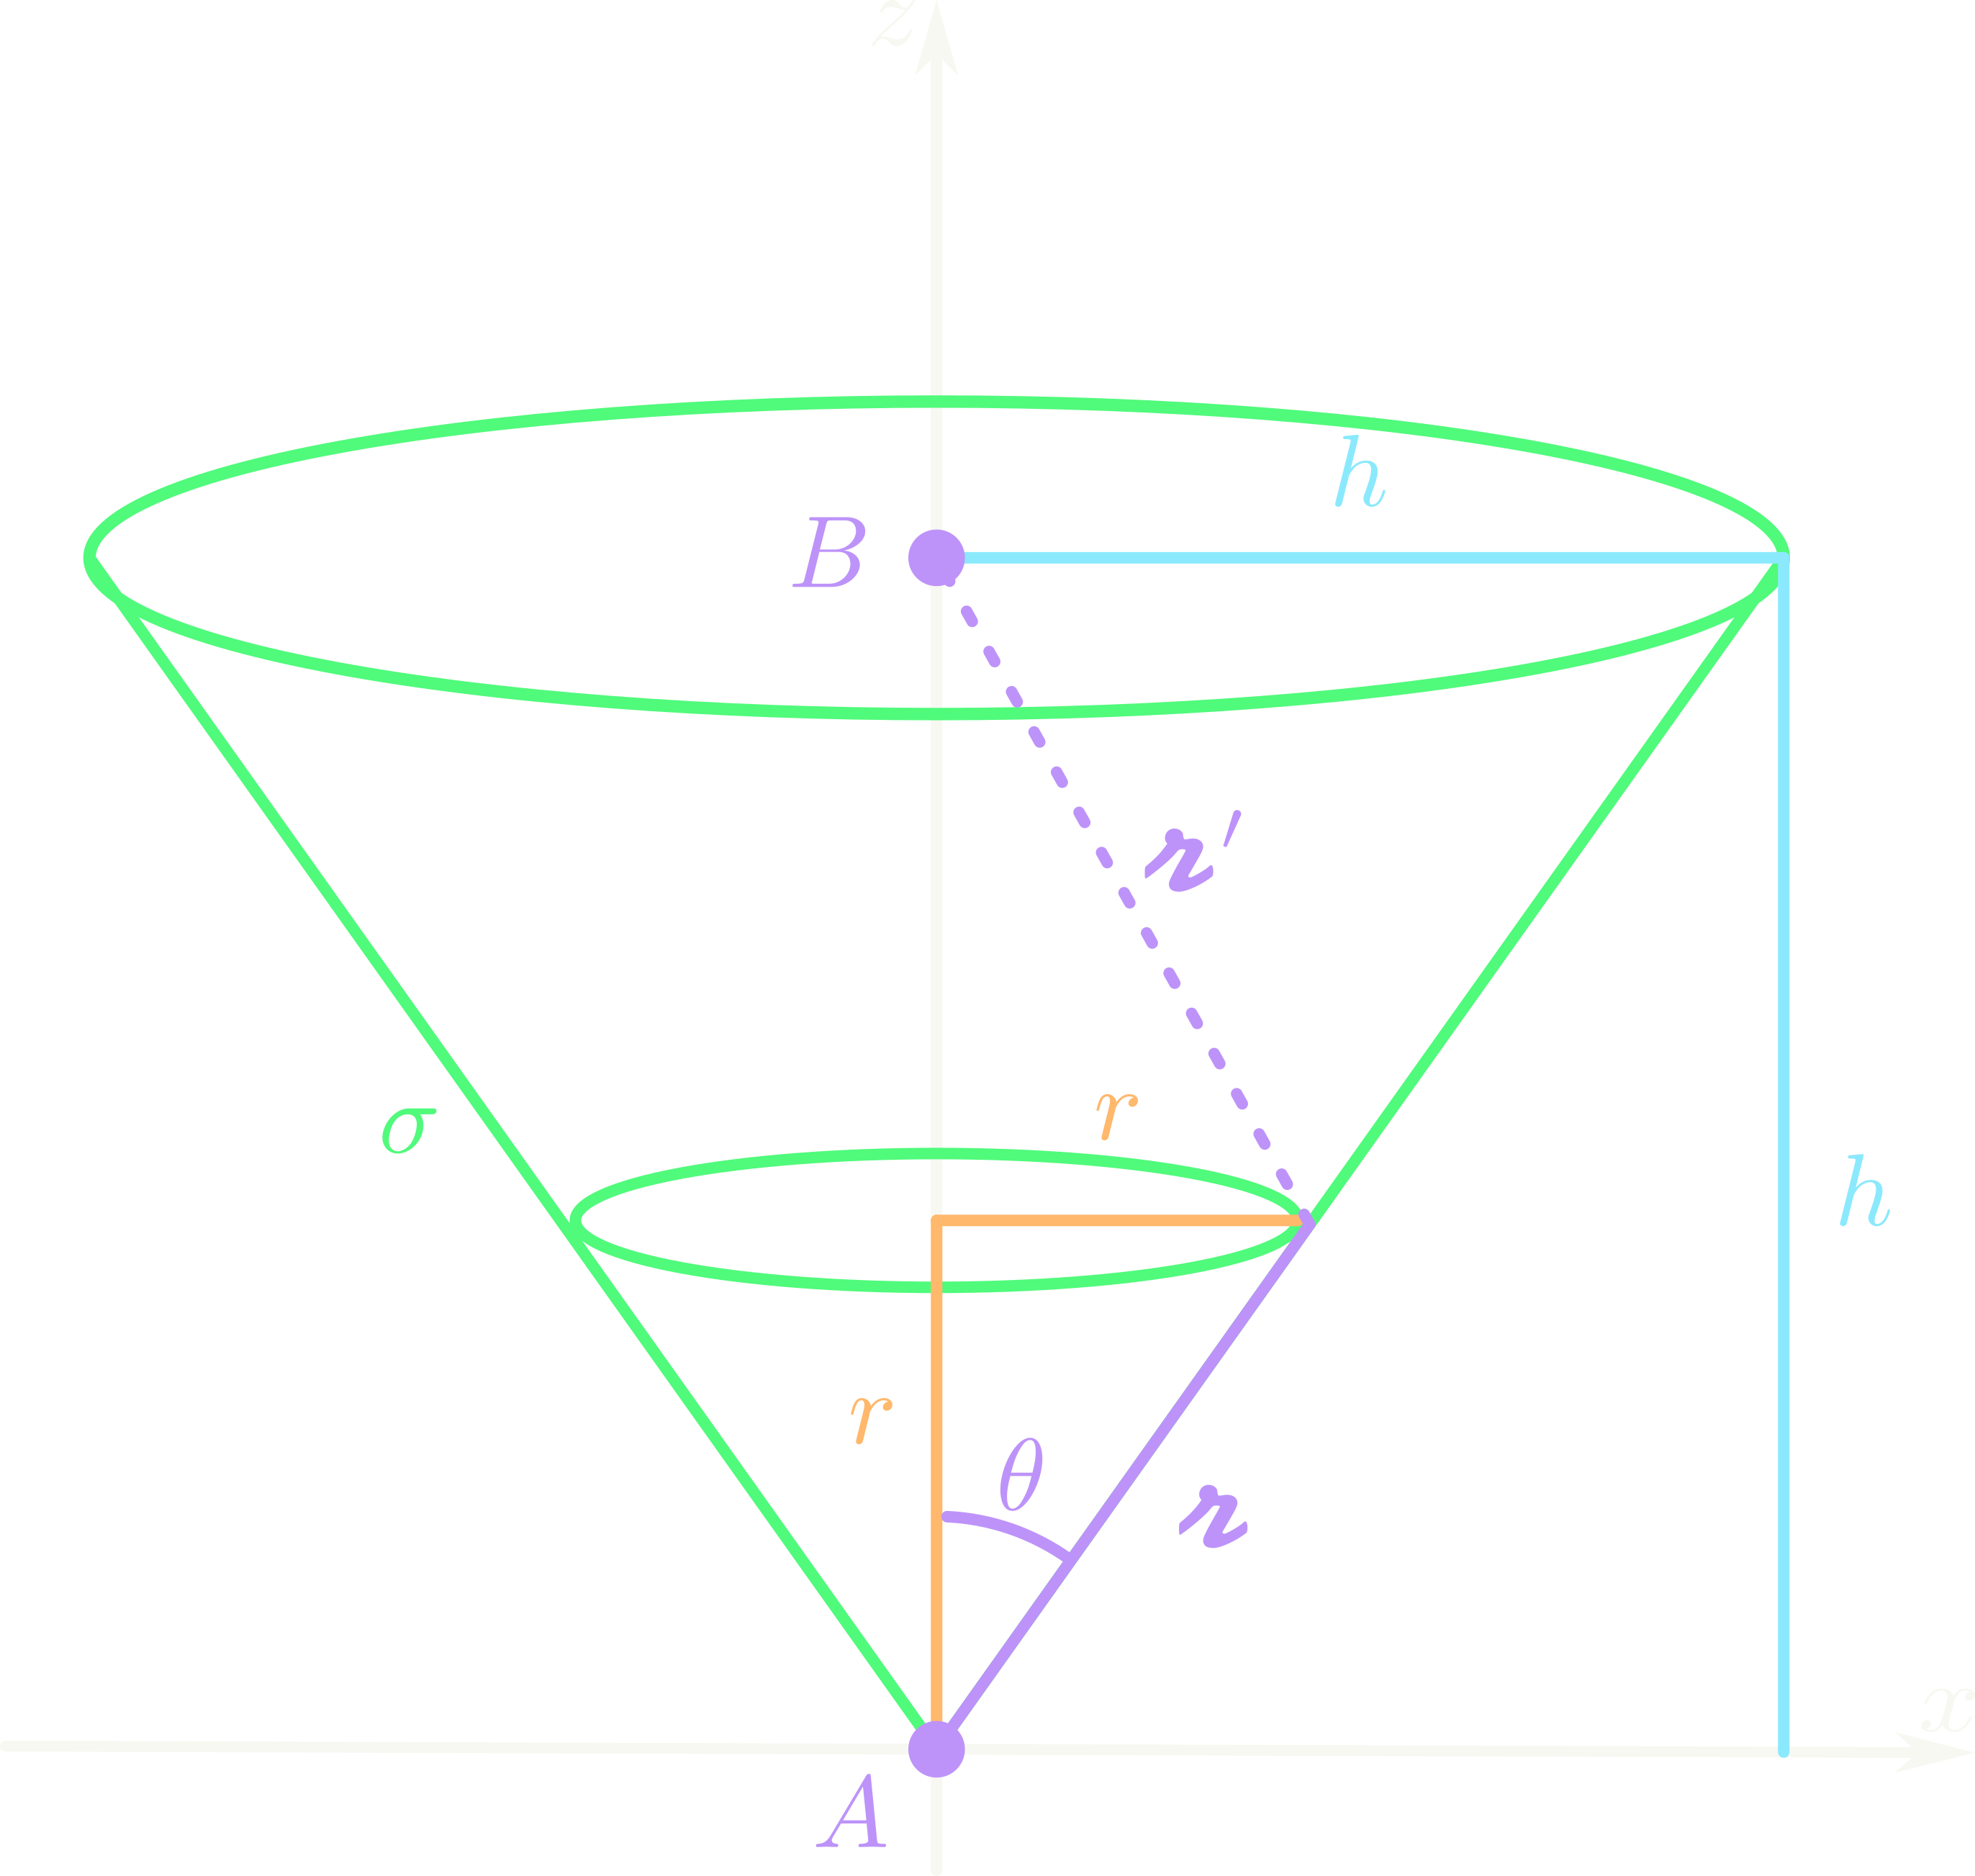
\includegraphics[width=0.5\linewidth]{images/hw2_26.png}
    \captionsetup{width=0.8\linewidth}
    \caption{Empty ice cream cone with surface charge density $\sigma$.}
    \label{fig:2_26}
\end{figure}
\begin{itemize}
    \item [(i)] Potential at $A$: Geometrically, we can see from the large right triangle that
    \begin{align*}
        \scriptr^2 = h^2 + h^2 \\
        \implies \scriptr = h\sqrt{2}, \quad h = \frac{\scriptr}{\sqrt{2}}
    \end{align*}
    and from the smaller right triangle
    \begin{align*}
        \scriptr^2 = 2r^2 \implies r = \frac{\scriptr}{\sqrt{2}}
    \end{align*}
    We can find the potential at $A$ using Eq. \eqref{eq:2_30} and integrate the rings of the cone along the slant length $0 \to h\sqrt{2}$
    which gives us the area element $\dd{a} = 2\pi r \dd{\scriptr}$:
    \begin{align*}
        V(A) &= \ke \int_0^{h\sqrt{2}} \frac{\sigma}{\scriptr} 2\pi r \dd{\scriptr} \\
        &= \frac{\sigma}{2\epsilon_0\sqrt{2}} \int_0^{h\sqrt{2}} \dd{\scriptr} \\
        &= \frac{\sigma}{2\epsilon_0\sqrt{2}} \scriptr \eval_0^{h\sqrt{2}} \\
        V(A) &= \frac{\sigma h}{2\epsilon_0}
    \end{align*}

    \item[(ii)] Potential at $B$: Using the law of cosines,
    \begin{align*}
        \scriptr'^2 = h^2 + \scriptr^2 - 2h\scriptr\cos\theta
    \end{align*}
    where
    \begin{align*}
        \cos\theta &= \frac{h}{\scriptr} \\
        &= \frac{h}{h\sqrt{2}} = \frac{1}{\sqrt{2}} = \frac{\sqrt{2}}{2} \\
        \implies \scriptr' &= \sqrt{h^2 + \scriptr^2 - h\scriptr\sqrt{2}}
    \end{align*}
    so the potential at $B$ is
    \begin{align*}
        V(B) &= \ke \int_0^{h\sqrt{2}} \frac{\sigma}{\scriptr'} 2\pi r \dd{\scriptr} \\
        &= \frac{\sigma}{2\epsilon_0\sqrt{2}} \int_0^{h\sqrt{2}} \frac{\scriptr}{\sqrt{h^2 + \scriptr^2 - h\scriptr\sqrt{2}}} \dd{\scriptr}
    \end{align*}
    I just used integral-calculator for this one\dots
    \begin{align*}
        V(B) &= \frac{\sigma}{2\epsilon_0\sqrt{2}} \qt[h\sqrt{2} \ln(1 + \sqrt{2})] \\
        V(B) &= \frac{\sigma h}{2\epsilon_0} \ln(1 + \sqrt{2})
    \end{align*}
    Finally the potential difference between $A$ and $B$ is
    \begin{align*}
        V(B) - V(A) = \frac{\sigma h}{2\epsilon_0} \ln(1 + \sqrt{2}) - \frac{\sigma h}{2\epsilon_0} \\
        \boxed{V(B) - V(A) = \frac{\sigma h}{2\epsilon_0} \qt[\ln(1 + \sqrt{2}) - 1]}
    \end{align*}
\end{itemize}

\paragraph{2.34} For a solid sphere radius $R$ and charge $q$
\begin{itemize}
    \item [(a)] From Problem \nameref{prob:2_21}
    \begin{align*}
        V = \ke \frac{q}{2R} \qt(3 - \frac{r^2}{R^2}) 
    \end{align*} and
    \begin{align*} \tag{2.43} \label{eq:2_43}
        W = \frac{1}{2} \int \rho V \dd{\tau}
    \end{align*}
    So the energy is 
    \begin{align*}
        W &= \frac{\rho}{2} \ke \frac{q}{2R} \int_0^{2\pi}\int_0^\pi\int_0^R \qt(3 - \frac{r^2}{R^2}) r^2 \sin\theta \dd{r} \dd{\theta} \dd{\phi} \\
        &= \frac{\rho}{2} \ke \frac{q}{2R} 4\pi \int_0^R \qt(3r^2 - \frac{r^4}{R^2}) \dd{r} \\
        &= \frac{\rho q}{4R\epsilon_0} \qt[r^3 - \frac{r^5}{5R^2}]_0^R \\
        &= \frac{\rho q}{4R\epsilon_0} \qt[R^3 - \frac{R^3}{5}] \\
        &= \frac{\rho q}{5\epsilon_0} R^2
    \end{align*}
    where the charge over the volume of the sphere is $\rho = \frac{q}{\frac{4}{3}\pi R^3}$, thus
    \begin{align*}
        W = \frac{q}{5\epsilon_0} R^2 \frac{q}{\frac{4}{3}\pi R^3} \\
        \boxed{W = \ke \frac{3q^2}{5R}}
    \end{align*}
    \item[(b)] Integrating over all space using 
    \begin{align*}\tag{2.45} \label{eq:2_45}
        W = \frac{\epsilon_0}{2} \int E^2 \dd{\tau}
    \end{align*}
    Where the electric field is
    \begin{align*}
        \vb{E}_{out} = \ke \frac{q}{r^2} \vu{r} \quad \vb{E}_{in} = \ke \frac{q}{R^3} r \vu{r}
    \end{align*}
    so the energy is
    \begin{align*}
        W &= \frac{\epsilon_0}{2} \frac{1}{(4\pi\epsilon_0)^2} 4\pi q^2 \qt[\int_0^R \frac{r^2}{R^6} r^2 \dd r + \int_R^\infty \frac{1}{r^4} r^2 \dd r] \\
        &= \ke \frac{q^2}{2} \qt[\int_0^R \frac{r^4}{R^6} \dd r + \int_R^\infty \frac{1}{r^2} \dd r] \\
        &= \ke \frac{q^2}{2} \qt[\frac{r^5}{5R^6}\eval_0^R - \frac{1}{R}\eval_R^\infty] \\
        &= \ke \frac{q^2}{2} \qt[\frac{R^5}{5R^6} + \frac{1}{R}] \\
        &= \ke \frac{q^2}{2} \frac{6}{5R} \\
        W &= \ke \frac{3q^2}{5R}
    \end{align*}
    checkmark.
    \item[(c)] For a spherical volume of radius $a$ and
    \begin{align*} \tag{2.44} \label{eq:2_44}
        W &= \frac{\epsilon_0}{2} \qt(\int_V E^2 \dd\tau + \oint_S V \vb E \cdot \dd\vb a)
    \end{align*}
    we can assume the volume is outside the charged sphere so
    \begin{align*}
        V &= \ke \frac{q}{r}
    \end{align*}
    From part (b), the first term is
    \begin{align*}
        \frac{\epsilon_0}{2} \int_V E^2 \dd\tau &= \ke \frac{q^2}{2} \qt[\frac{1}{5R} - \frac{1}{a} + \frac{1}{R}] \\
        &= \ke \frac{q^2}{2} \qt[\frac{6}{5R} - \frac{1}{a}]
    \end{align*}
    the second term is at $r = a$
    \begin{align*}
        \frac{\epsilon_0}{2} \oint_V V \vb E \cdot \dd\vb a &= \frac{\epsilon_0}{2} \frac{1}{(4\pi\epsilon_0)^2} \int \frac{q}{r} \frac{q}{r^2} r^2 \sin\theta \dd \theta \dd\phi \\
        &= \frac{4\pi\epsilon_0}{2} \frac{1}{(4\pi\epsilon_0)^2} \frac{1}{r} \eval_{r = a} \\
        &= \ke \frac{q^2}{2a}
    \end{align*}
    so the total energy is
    \begin{align*}
        W &= \ke \frac{q^2}{2} \qt[\frac{6}{5R} - \frac{1}{a}] + \ke \frac{q^2}{2a} \\
        &= \ke \frac{3q^2}{5R} 
    \end{align*}
    As $a \to \infty$ the $\int V\vb E \cdot \dd\vb a$ term goes to zero.
\end{itemize}

\paragraph{2.39} Two cavities radii $a$ and $b$ in a conducting sphere of radius $R$ with a point charge $q_a$ and $q_b$ respectively in each cavity.
\begin{itemize}
    \item [(a)] Surface charge densities:
    
    On the surface of cavity $a$ the charge density is simply
    \begin{align*}
        \sigma_a = \frac{-q_a}{4\pi a^2}
    \end{align*}
    and 
    \begin{align*}
        \sigma_b = \frac{-q_b}{4\pi b^2}
    \end{align*}
    respectively. For the surface of the conducting sphere, the charge density is positive and equal to the superposition of the two charges:
    \begin{align*}
        \sigma_R = \frac{q_a + q_b}{4\pi R^2}
    \end{align*}
    \item [(b)] The field outside the conductor is equivalent to a point charge at the center of the sphere with the sum of the charges:
    \begin{align*}
        \vb E = \ke \frac{q_a + q_b}{r^2} \vu r
    \end{align*}
    \item [(c)] The field in cavity $a$ with respect to the center of the cavity is
    \begin{align*}
        \vb E_a = \ke \frac{q_a}{a^2} \vu a
    \end{align*}
    and in cavity $b$ is
    \begin{align*}
        \vb E_b = \ke \frac{q_b}{b^2} \vu b
    \end{align*}
    \item [(d)] The field due to to the cavity charge is zero in the exterior of the cavity, so there is no Force on $q_a$ or $q_b$.
    \item [(e)] If a charge $q_c$ was brought near the conductor from outside, there would be a change in (a) $\sigma_R$ and (b) $\vb E_{out}$.
\end{itemize}

\paragraph{2.47} Net force of of the southern hemisphere extering on the northern hemisphere (solid sphere) with an inside Electric field (Problem 2.8)
\begin{align*}
    E_{in} = \ke \frac{Q}{R^3} \vb r 
\end{align*}
where the total force is 
\begin{align*}
    \vb F = Q \vb E = \ke \frac{Q^2}{R^3} \vb r
\end{align*}
Finding the net force exerted by the southern hemisphere: integrate $\dd F = \vb F / V$ over the southern hemisphere:
\begin{align*}
    \dd F &= \frac{1}{\frac{4}{3} \pi R^3} \ke \frac{Q^2}{R^3} \vb r \dd \tau \\
    &= \frac{3Q^2}{16\pi^2 \epsilon_0 R^6} \vb r \dd \tau
\end{align*}
The symmetry of the sphere implies that the Force is only in the $z$-direction i.e. $F_z = F \cos\theta$, so integrating over the southern hemisphere:
\begin{align*}
    \int_0^{2\pi} \int_0^{\pi/2} \int_0^R F_z \dd \tau &= \frac{3Q^2}{16\pi^2 \epsilon_0 R^6} \int_0^{2\pi} \int_0^{\pi/2} \int_0^R r \cos\theta r^2 \sin \theta \dd r \dd \theta \dd \phi \\
    &= \frac{3Q^2}{16\pi^2 \epsilon_0 R^6} (2\pi) \qt(\frac{r^4}{4})\eval_0^R \int_0^{\pi/2} \sin\theta \cos\theta \dd \theta \dd \phi \\
    &= \frac{3Q^2}{32\pi \epsilon_0 R^2} \frac{\sin^2 x}{2} \eval_0^{\pi/2} \\
    &= \boxed{\frac{3Q^2}{64\pi \epsilon_0 R^2}}
\end{align*}

\subsubsection*{USE GRIFFITHS 5th EDITION FROM NOW ON}
\end{document}